\documentclass[a4paper, 11pt, onecolumn, twoside, openright]{report}

\usepackage[french]{babel}
\usepackage{color}
\usepackage{frbib}
\usepackage{booktabs}
\usepackage[T1]{fontenc}
\usepackage{amsfonts}
\usepackage{lettrine}
\usepackage{times}
\usepackage[Lenny]{fncychap}
\usepackage{graphicx}
\usepackage{hyperref}
\usepackage{cleveref}
\usepackage{times}
\usepackage{amstext}
\usepackage{subfigure}
\usepackage{heiglogo}
\usepackage{listings}

\lstset{language=C}
\lstset{basicstyle=\scriptsize\ttfamily, stringstyle=\ttfamily}
\lstset{tabsize=2,showstringspaces=false}

\newcommand{\ccode}[1]{{\lstset{basicstyle=\normalsize\ttfamily,stringstyle=\ttfamily}\lstinline$#1$}}

\usepackage[chapter]{algorithm}
\usepackage{algorithmic}
\usepackage{tabularx}
\usepackage{fancyhdr}

\usepackage{ulem}

\normalem

\usepackage[labelfont=bf,justification=justified,format=hang,skip=0pt,nooneline]{caption}

\floatname{algorithm}{Algorithme}

\graphicspath{{./images/}}


\newcommand{\com}[1]{}
%\renewcommand{\com}[1]{\pagebreak{\typeout{Comment: #1}\Huge\textbf{#1}}\pagebreak}


\newcommand{\ang}[1]{\textit{#1}}

%\renewcommand{\includegraphics}[2]{}


\setlength{\headheight}{1.2cm}

\setlength{\voffset}{-1.2cm}

\setlength{\textheight}{655pt}


\addtolength{\oddsidemargin}{-1cm}
\addtolength{\evensidemargin}{-1cm}
\addtolength{\textwidth}{2cm}

\newcounter{exercicecounter}
\setcounter{exercicecounter}{1}

\newcommand{\extitle}[1]{\begin{center}{\Huge #1}\end{center}\vspace{1cm}}

\newenvironment{exercice}[1][]{{%
  \noindent%
  \begin{minipage}[l]{\linewidth}%
    \vspace{8mm}%
    \rule{\linewidth}{0.2mm} \\%
    %%\vspace{1mm}%
    \large\textbf{Exercice \theexercicecounter :} #1\\ %
    \rule{\linewidth}{0.2mm}%
    \vspace{5mm}%
    \addtocounter{exercicecounter}{1}%
  \end{minipage}}}{}

\newcommand{\startexercice}{\subsection*{Exercice \thechapter.\theexercicecounter}\addtocounter{exercicecounter}{1}}

\newcommand{\startchapter}{\thispagestyle{myplain}
%\setcounter{page}{1}
\setcounter{exercicecounter}{1}}

\setlength{\unitlength}{1cm}

\pagestyle{fancy}
% with this we ensure that the chapter and section
% headings are in lowercase
\renewcommand{\chaptermark}[1]{\markboth{\MakeUppercase{\chaptername}\ \thechapter.\ \MakeUppercase{#1}}{}}
%\renewcommand{\rightmark}[1]{PCO1. \markboth{\MakeUppercase{\chaptername}\ \thechapter.\ \MakeUppercase{#1}}{}}
%\renewcommand{\chaptermark}[1]{PCO1. \markboth{\MakeUppercase{\chaptername}\ \thechapter.\ \MakeUppercase{#1}}{}}
\fancyhf{} %delete the current section for header and footer
\renewcommand{\headrulewidth}{0pt}
\fancyhead[RO]{\thepage}
\fancyhead[LE]{\thepage}
\fancyhead[LO]{\rightmark}
\fancyhead[RE]{\leftmark}
%\fancyfoot[C]{Programmation Concurrente 1 \copyright HEIG-VD}
\fancyheadoffset[LE,RO]{1.5cm} \fancyfootoffset[LE,RO]{1.5cm}
%\fancyhead[LE]{{\Roman{chapter}}.\thepage}

\fancypagestyle{myplain}{%
%\fancyhf{} % clear all header and footer fields
\renewcommand{\headrulewidth}{0pt}
\fancyhead{}
%\fancyfoot[C]{Programmation Concurrente 1 \copyright HEIG-VD}
}

\renewcommand{\figurename}{Figure}
\def\listfigurename{Liste des figures}
\renewcommand{\tablename}{Tableau}


\emergencystretch=50pt

\renewcommand{\labelitemi}{$\bullet$}

\setcounter{tocdepth}{2}
\setcounter{secnumdepth}{2}

\setlength{\parindent}{0pt}

\begin{document}


\begin{titlepage}

\logo{1cm}{1cm}
\centering \scshape \vspace*{\fill}

{\Huge Introduction à la\\\vspace{1em}Programmation Concurrente} \vspace{5em}

{\Large Polycopié du cours PCO} \vspace{5em}

\upshape

{\Large Prof. Claude Evéquoz, Prof. Yann Thoma, Prof. Yves Chevallier }
\vspace{2em}

{\Large
HEIG-VD\\
2023}

\vspace*{\fill}

\end{titlepage}

\thispagestyle{empty} \thispagestyle{empty}

\addcontentsline{toc}{chapter}{Table des matières}
\tableofcontents

\chapter{Introduction à la programmation concurrente}\label{sec:into}
\startchapter

\section{Qu'est-ce que la programmation concurrente?}


\lettrine[lines=4]{E}{n programmation} séquentielle, un programme est décomposé en sous-programmes (procédures ou fonctions). Chaque sous-programme correspond à une suite d'instructions, et l'exécution du programme voit ces instructions être exécutées les unes à la suite des autres. Les premiers ordinateurs (et leurs successeurs durant quelques années) ont fonctionné selon ce mode d'exécution sérielle. Une tâche pouvait en appeler une autre, mais la tâche appelante ne continuait son exécution qu'après la terminaison de la tâche appelée. Cette approche, simple à mettre en oeuvre en comparaison des systèmes actuels, souffre toutefois de quelques faiblesses. Un seul programme peut être exécuté à la fois, ce qui interdit entre autres à un utilisateur de travailler sur un document en même temps qu'il compile un code source. Si le programme en cours d'exécution attend que l'utilisateur effectue une action (clic souris par exemple), alors le processeur se retrouve sous-exploité. Et enfin, si un programme engendre une erreur, et se fige, alors le système risque de se retrouver totalement bloqué.

À l'heure actuelle, les systèmes informatiques sont multiprocessus, et supportent l'exécution pseudo-parallèle de plusieurs processus (programmes en exécution). Ceci a été rendu possible par la mise au point de systèmes d'exploitation nettement plus complexes. Un processeur peut donc voir plusieurs processus en cours d'exécution se partager le temps de traitement. Et de même, un processus peut être décomposé en sous-processus ou \emph{tâche} (\emph{threads} en anglais). Ces threads permettent de ne plus être liés à une exécution totalement sérielle des instructions. Il est dès lors possible d'avoir, par exemple, un thread responsable d'exécuter un calcul lourd pendant qu'un autre gère les interactions avec l'utilisateur. Un serveur FTP, par exemple, peut plus facilement gérer plusieurs connexions simultanées, chaque connexion étant gérée par un thread.


\section{Parallélisme vs. concurrence}

Le terme \emph{programmation concurrente} ne doit pas être confondu avec celui de \emph{programmation parallèle} (ou programmation répartie). La programmation concurrente, telle que nous l'entendrons, se réfère à un système décomposé en tâches pouvant être exécutées dans un ordre quelconque. Certaines tâches sont exécutées avant d'autres, et certaines le sont en parallèle. La programmation parallèle traite, quant à elle, de l'exécution simultanée de tâches sur différents processeurs. Il s'agit alors de pouvoir synchroniser des processus entre eux, ceci principalement au travers d'une mémoire partagée ou de liaisons réseau.

Dans le cadre de ce cours, nous ne traiterons pas de la communication interprocessus, mais bien de la communication intraprocessus. Un programme sera décomposé en threads, qui sont donc ses fils d'exécution pseudo-parallèles. Les problèmes qui vont nous intéresser sont donc le partage de données et la synchronisation entre threads. Il est intéressant de noter que le concept de programmation concurrente est autant valable sur un processeur simple cœur que sur un multicœur. Sur un simple cœur, les parties de threads s'exécutent tour à tour de manière transparente, et sur un multicœur, un réel parallélisme peut être observé, chaque cœur pouvant exécuter un ensemble de threads.

L'illustration de la programmation concurrente sera faite par le biais de 2 langages. Le premier, le langage C, n'offre dans sa définition aucun mécanisme concurrent. Pour contourner ce problème, nous allons utiliser la bibliothèque standard \emph{pthread}, qui propose un ensemble de mécanismes pour la gestion des threads. Elle permet de décrire une application sous forme d'un ensemble de threads, ces threads étant ensuite exécutés sur la machine cible. Le second langage, Java, quant à lui, met à disposition la notion de threads et quelques mécanismes rudimentaires. Ce langage ne sera pas traité dans ce cours.

\section{Anatomie d'un processus}

Un processus correspond à un fichier exécutable en cours d'exécution sur un processeur. Il est entre autres caractérisé par un code (le programme à exécuter), une pile et un tas qui permettent de stocker les données nécessaires à son bon fonctionnement, un identifiant unique, et une priorité. La priorité permet au système d'exploitation de gérer plusieurs processus en cours d'exécution sur un processeur, un processus à plus haute priorité se voyant attribuer un temps d'utilisation de processeur plus important.

Un processus est créé lorsqu'un autre processus lance son exécution. Nous pouvons distinguer le processus parent (celui qui lance), et le processus enfant.

La figure \ref{fig:process-state-unix} illustre les différentes étapes de la vie d'un processus, pour un système d'exploitation de type Unix. L'état initial d'un processus est \emph{terminé} (\emph{destroyed} en anglais). Après sa création, il passe à l'état \emph{prêt} (\emph{ready} en anglais) lorsque toutes les ressources à son bon fonctionnement ont été réquisitionnées.
Le système d'exploitation peut ensuite le faire passer dans l'état \emph{élu}, (\emph{active} en anglais), état dans lequel le processus s'exécute.
Ce passage n'est pas du ressort du processus, mais bien de l'ordonnanceur, qui s'occupe d'allouer le processeur aux différents processus concurrents. À tout instant l'ordonnanceur peut replacer le processus dans l'état \emph{prêt}, pour laisser un autre processus s'exécuter. Il s'agit de la \emph{préemption} d'un processus, qui se fait sans que le processus préempté n'en soit conscient. Depuis l'état \emph{élu}, le processus peut aussi se retrouver dans l'état \emph{bloqué} (\emph{blocked} en anglais), lors de l'attente d'un événement ou du relâchement d'un mutex, par exemple. Il n'y a ensuite qu'une possibilité pour sortir de l'état \emph{bloqué}. Il s'agit de réveiller le processus suite au relâchement d'un mutex ou au fait qu'un événement sur lequel le processus attend a été déclenché. Dans ce cas, le processus passe à l'état \emph{prêt}, prêt à continuer son exécution. Lorsque le processus s'exécute, il peut se terminer. Les deux autres flèches sortantes de l'état \emph{élu} représentent deux scénarios. Premièrement, si le processus a été détaché, c'est-à-dire qu'il est sans lien parental, lors de sa terminaison, le processus passe directement dans l'état \emph{terminé}. Deuxièmement, si la terminaison du processus est importante pour le reste de l'application, alors il passe dans l'état \emph{zombie} (\emph{zombied} en anglais). Il y reste jusqu'à ce que le processus parent effectue une \emph{jointure}, c'est-à-dire qu'il récupère les informations retournées par le processus en cours de terminaison.

\begin{figure}[ht]
  \centering
  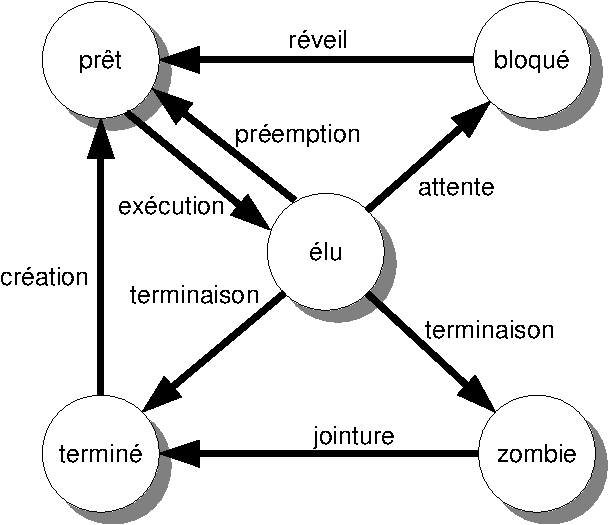
\includegraphics{images/process-state-unix}
  \caption{\label{fig:process-state-unix}États et transitions d'un processus Unix}

\end{figure}

La figure \ref{fig:process-space} illustre la décomposition de l'espace d'adressage d'un processus en trois parties principales~:
\begin{itemize}
  \item Le code contenant les instructions du programme (\emph{text segment} en anglais).
  \item Les variables globales et les variables allouées dynamiquement (\emph{data segment} en anglais).
  \item La pile, où les variables locales de ses sous-programmes, ainsi que diverses informations temporaires ayant une durée de vie égale au sous-programme sont stockées (\emph{stack segment} en anglais).
\end{itemize}

\begin{figure}[ht]
  \centering
  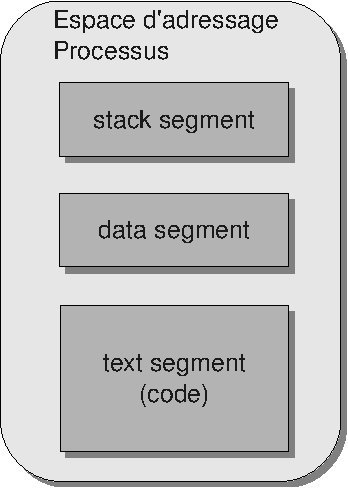
\includegraphics{process-space}
  \caption{\label{fig:process-space}Espace d'adressage d'un processus}

\end{figure}


Un processus, dans un cadre multithreadé, est décomposé en deux parties~:
\begin{itemize}
  \item La première contenant les ressources globales, telles que les instructions du programme et les variables globales. Cette partie correspond au \emph{processus}. Il s'agit des deux premiers points de l'espace d'adressage.
  \item La deuxième contenant des informations liées à l'état d'exécution, telles que le \emph{compteur de programme} (aussi appelé \emph{compteur ordinal}) et la \emph{pile d'exécution}. Cette partie correspond à un thread. Il est à noter que chaque thread possède un compteur de programme et une pile. Il s'agit de la partie liée au \emph{thread}.
\end{itemize}

\section{Anatomie d'un thread}

Un thread est un fil d'exécution de code, à l'intérieur d'un processus, et qui a la possibilité d'être ordonnancé. Il s'agit d'une version allégée d'un processus. Processus et threads partagent certaines propriétés, mais ne peuvent en aucun cas être interchangés. Tout processus a un thread principal, depuis lequel d'autres threads peuvent être lancés, dans le cas d'une application multithread.

Les threads d'un même processus partagent le même espace d'adressage, comme illustré à la figure \ref{fig:process-space-multi}. Toutes les ressources du processus peuvent être accédées par tous les threads, ce qui n'est pas le cas entre deux processus distincts. Toutefois, chaque thread possède son propre compteur de programme (PC), un ensemble de registres, un état, et une pile. Les piles sont placées dans l'espace mémoire dédié aux piles, mais chaque thread possède sa propre pile. Les variables globales sont par contre partagées entre les threads.

\begin{figure}[!ht]
  \centering
  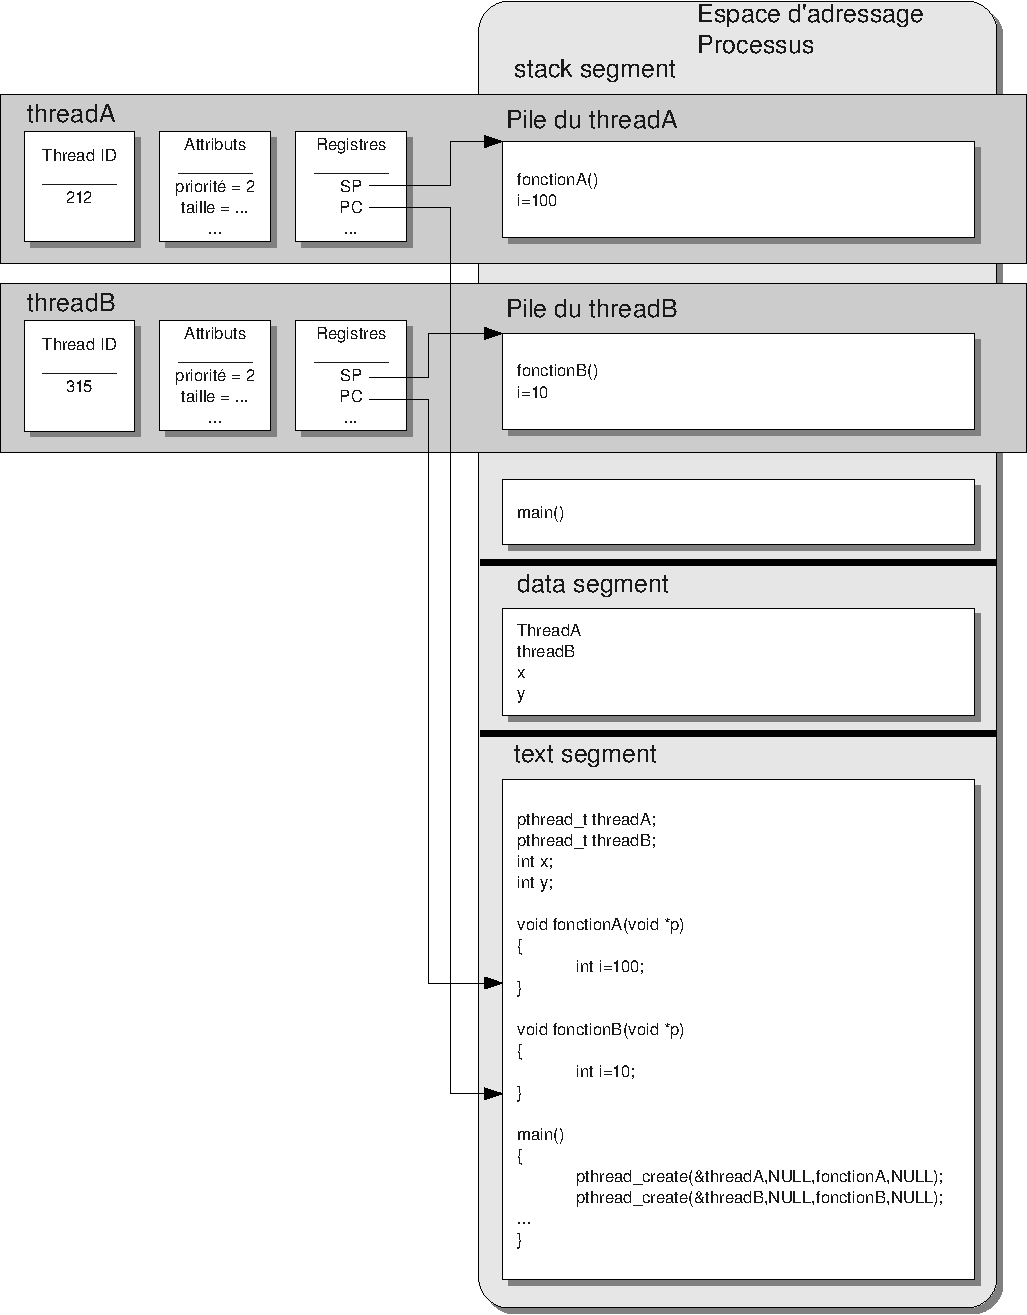
\includegraphics[width=\textwidth]{process-space-multi}
  \caption{\label{fig:process-space-multi}Espace d'adressage d'un processus multithread}

\end{figure}

Du point de vue du programmeur, le programme de la figure \ref{fig:process-space-multi} s'exécute à la manière présentée sur la figure \ref{fig:thread-execution}.

\begin{figure}[ht]
  \centering
  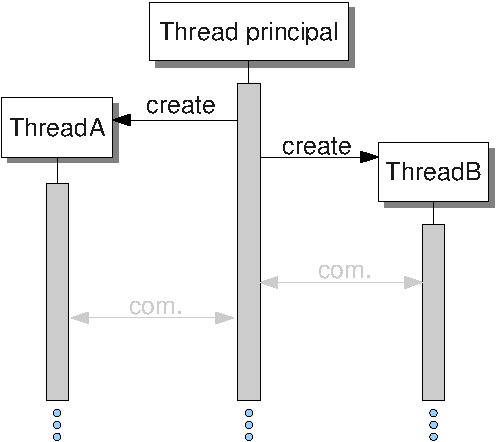
\includegraphics{thread-execution}
  \caption{\label{fig:thread-execution}Flot d'exécution d'un processus multithread}

\end{figure}

Toutefois, sur un processeur simple cœur, les threads doivent se partager le processeur. De ce fait, le flot d'exécution ressemble plutôt à celui présenté sur la figure \ref{fig:thread-execution-single}. Nous pouvons observer qu'un seul thread est en exécution à un instant donné, et que le passage d'un thread à un autre peut être influencé par une communication interthread (deux derniers cas), ou simplement dicté par l'ordonnanceur.

\begin{figure}[ht]
  \centering
  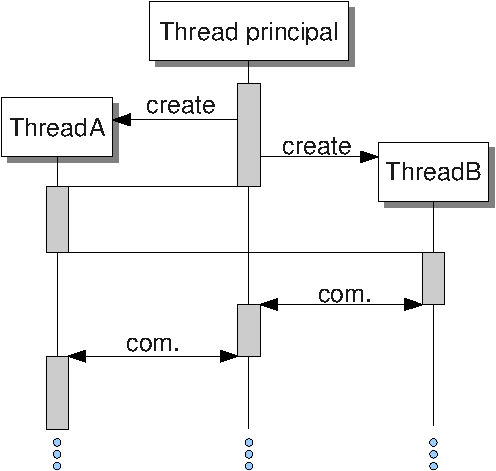
\includegraphics{thread-execution-single}
  \caption{\label{fig:thread-execution-single}Flot d'exécution d'un processus multithread sur un processeur simple cœur}

\end{figure}

Le cycle de vie d'un thread est semblable à celui d'un processus (figure \ref{fig:process-state-unix}).

Bien que la programmation multithread offre, dans le cadre de la programmation concurrente, passablement d'avantages sur la programmation multiprocessus, il faut être conscient des dangers y relatifs~:

\begin{itemize}
  \item Étant donné que les threads d'un même processus partagent le même espace d'adressage, un thread peut facilement corrompre les données utilisées par un autre thread. Des outils de synchronisation permettent toutefois d'éliminer les risques de ces corruptions, s'ils sont utilisés de manière appropriée.

  \item Toujours lié au partage de l'espace d'adressage, si un thread effectue un accès mémoire erroné fatal, le processus entier risque de se terminer. Ce n'est évidemment pas le cas pour un système à plusieurs processus.

  \item Un thread est lié à un programme particulier, et ne peut donc pas être lancé par un autre programme. Les processus peuvent en revanche être lancés par un autre processus, et donc être plus aisément réutilisés.
\end{itemize}

Pour résumer, listons ce que les processus et les threads ont en commun ou non.

En commun~:
\begin{itemize}
  \item possèdent un identifiant (ID), un ensemble de registres, un état, et une priorité;
  \item possèdent un bloc d'information;
  \item partagent des ressources avec les processus parents;
  \item sont des entités indépendantes, une fois créées;
  \item les créateurs du processus ou du thread ont contrôle sur eux;
  \item peuvent changer leurs attributs après création et créer de nouvelles ressources;
  \item ne peuvent accéder aux ressources d'autres threads et processus non reliés.
\end{itemize}

Pas en commun~:
\begin{itemize}
  \item les processus ont un espace d'adressage, les threads pas;
  \item les processus parents et enfants doivent utiliser des mécanismes de communication interprocessus; les threads d'un même processus communiquent en lisant et modifiant les variables de leur processus;
  \item les processus enfants n'ont aucun contrôle sur les autres processus enfants; les threads d'un processus sont considérés comme des pairs et peuvent exercer un contrôle sur les autres threads du processus;
  \item les processus enfants ne peuvent pas exercer de contrôle sur le processus parent; n'importe quel thread peut exercer un contrôle sur le thread principal, et donc sur le processus entier.
\end{itemize}


\section{Avantages du multithreading}

En comparaison d'un programme ne contenant qu'un seul thread, un programme décomposé en threads permet de mieux gérer les entrées/sorties et le calcul. Un thread peut s'occuper du calcul, tandis que d'autres gèrent les entrées/sorties. De ce fait, l'usage d'un GUI (Graphical User Interface) est plus ergonomique et convivial. Prenons l'exemple d'une application visant à afficher la courbe de Mandelbrot (Figure \ref{fig:mandelbrot}). Pour chaque point de l'image, une grande quantité de calcul doit être effectuée. Supposons que l'utilisateur peut cliquer sur des boutons pour zoomer. Si nous ne disposons pas de multithreading, un clic sur le bouton va ensuite voir l'application se bloquer pendant que la nouvelle image est calculée. Si par contre nous disposons de plusieurs threads, un thread peut s'occuper du calcul pendant que l'autre gère l'interface graphique. Dès lors l'utilisateur a encore la possibilité d'interagir avec l'application sans devoir souffrir de l'accaparement du processeur pour le calcul.

\begin{figure}[ht]
  \centering
  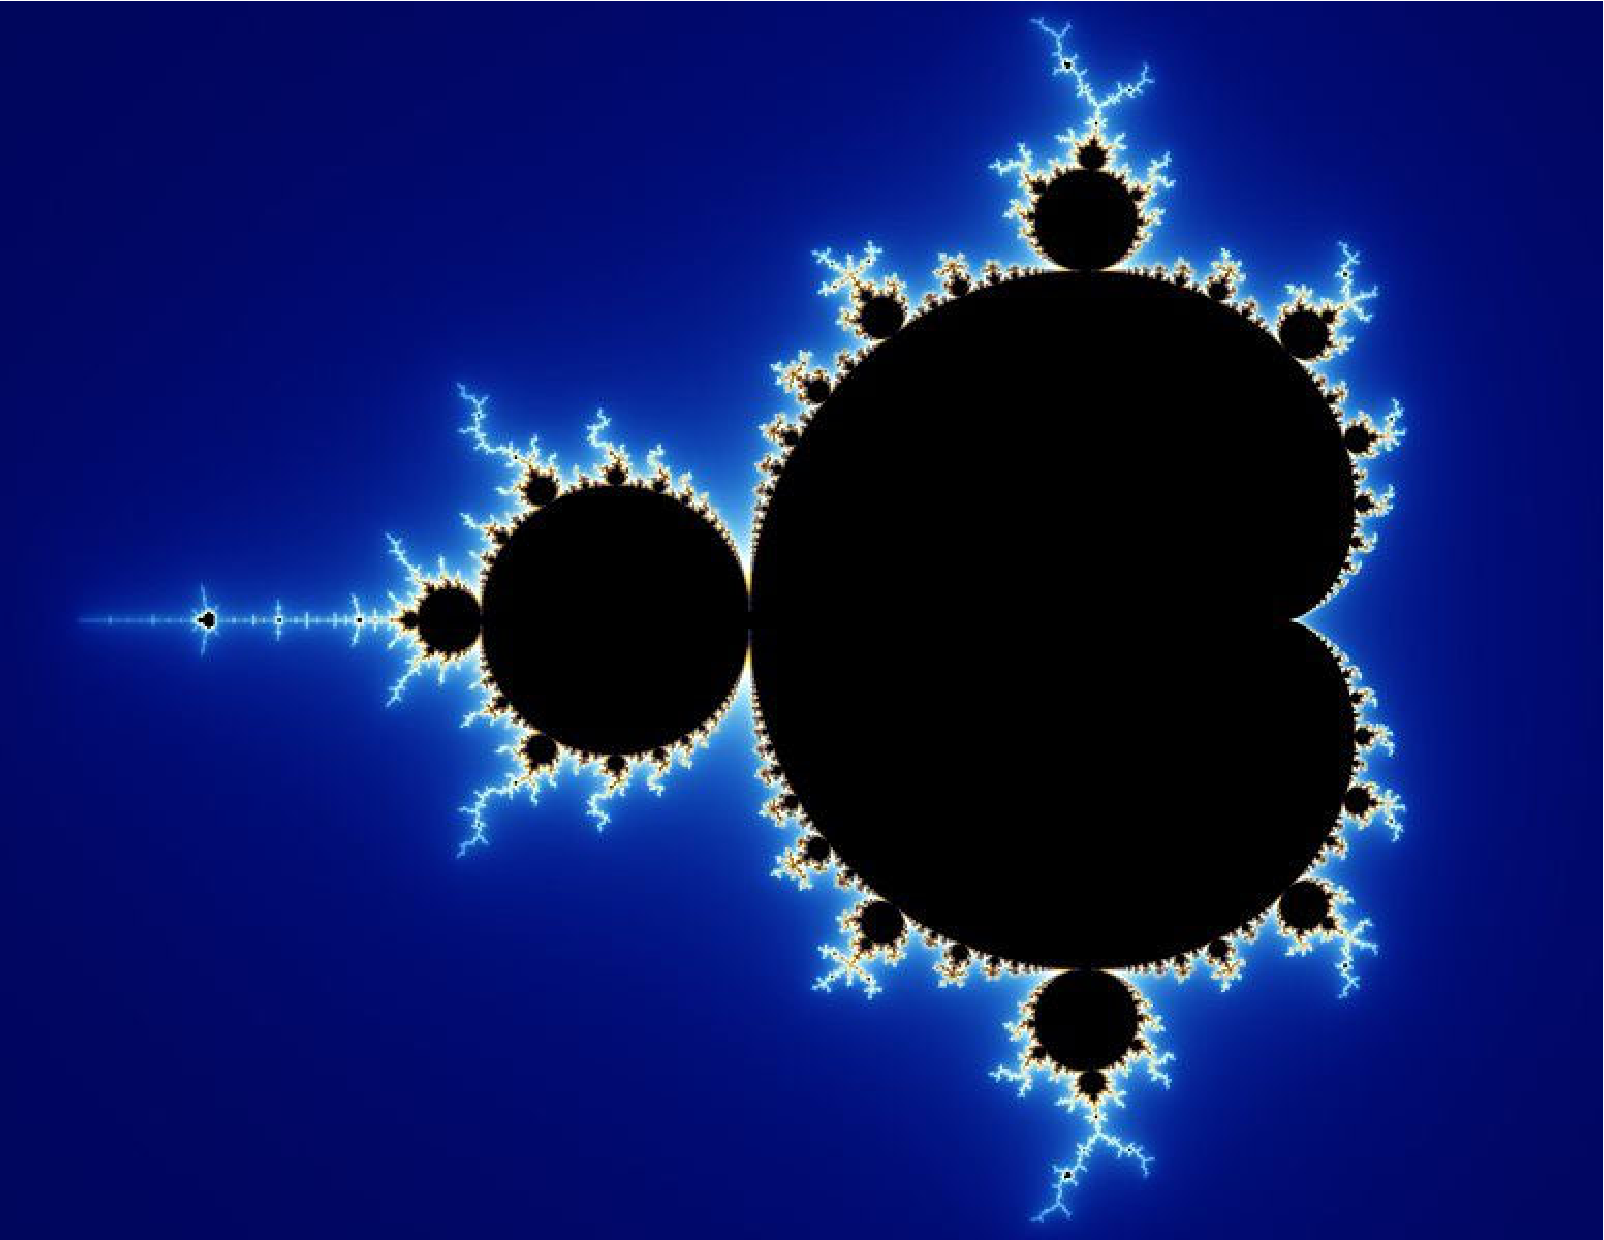
\includegraphics[width=.7\textwidth]{mandelbrot_image}
  \caption{\label{fig:mandelbrot}Courbe de Mandelbrot}

\end{figure}

Dans le cas d'un processeur multicœur, un autre avantage du multithreading peut s'exploiter. En effet, chaque cœur peut prendre en charge un ou plusieurs threads. En reprenant l'exemple de Mandelbrot, si nous supposons que nous sommes en présence d'un dual-core, alors nous pouvons décomposer notre calcul en deux threads, chacun étant responsable de la génération de la moitié de l'image. Lorsque l'utilisateur clique sur le bouton, la nouvelle image pourra donc s'afficher en un temps réduit de moitié. Il s'agit là d'un parallélisme réel, rendu possible par l'amélioration des plateformes matérielles proposées sur le marché. Nous pouvons toutefois noter que l'accélération d'un facteur $n$ pour un $n$-core reste théorique, la probable communication interthread imposant une perte en performance.

En comparaison d'un système multiprocessus, une application multithread requiert une surcharge (overhead) moindre pour la gestion des tâches. En effet, commuter d'un thread à un autre est nettement moins coûteux en termes de temps processeur que de commuter d'un processus à un autre. Un avantage d'une application multiprocessus est la possibilité d'exécuter les processus sur des machines différentes, ce qui n'est pas le cas du multithread. Pour ce qui est de la commutation, le responsable de son fonctionnement, dans les deux cas, est le système d'exploitation.

La table suivante (tirée de \cite{hughes03parallel}) liste les avantages et les inconvénients du multithreading par opposition au multi-processing~:

\begin{table}[ht]
  \begin{center}
    \caption{\label{tab:thread-vs-process}Avantages et inconvénients du multithreading par opposition au multi-processing}
    \begin{tabular}{p{.5\textwidth}p{.5\textwidth}}
      \toprule
      \textbf{Avantage des threads}                                         & \textbf{Désavantages des threads}                                            \\
      \midrule
      Moins de ressources nécessaires lors d'un changement de contexte      & Requiert des mécanismes de synchronisation lors d'accès mémoires concurrents \\
      Améliore le débit de traitement des données dans une application      & Peut facilement polluer l'espace d'adressage du processus                    \\
      Ne nécessite pas de mécanismes spéciaux de communication entre tâches & N'existe que dans un processus, et n'est donc pas réutilisable               \\
      Permet de simplifier la structure d'un programme                      &                                                                              \\
      \bottomrule
    \end{tabular}
  \end{center}
\end{table}

\section{Séparation d'un programme en plusieurs threads}

A priori, n'importe quelle application pourrait être réalisée à l'aide d'un seul thread. Toutefois, comme nous l'avons vu, cette approche est quelque peu limitée. Il faut alors se poser la question concernant la meilleure manière de décomposer une application. Nous pouvons identifier différents types de modèles, qui définissent la façon dont les threads interagissent entre eux:

\begin{itemize}
  \item Le modèle \emph{délégation} (\emph{boss-worker model} ou \emph{delegation model} en anglais)
  \item Le modèle \emph{pair} (\emph{peer model} en anglais)
  \item Le modèle \emph{pipeline} (\emph{pipeline model} en anglais)
\end{itemize}

\subsection{Modèle délégation}

Dans le modèle \emph{délégation} (Figure \ref{fig:model-boss-worker}), un thread principal s'occupe de répartir la charge de travail sur les threads travailleurs. Ce pourrait typiquement être le cas d'un serveur FTP où un thread attend des commandes et les délègue ensuite aux autres threads. La réalisation d'une application selon ce modèle peut se faire de deux manières.


\begin{figure}[ht]
  \begin{center}
    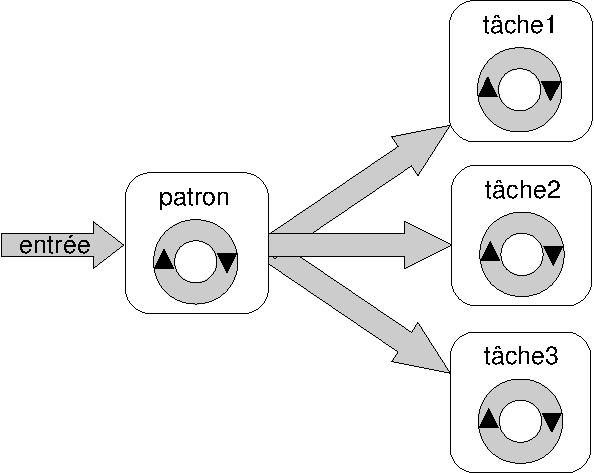
\includegraphics[scale=0.7]{model-boss-worker}
    \caption{\label{fig:model-boss-worker}Modèle délégation}
  \end{center}
\end{figure}

Premièrement, le thread principal peut créer un thread pour chaque nouvelle tâche à exécuter. Dans ce cas, il est composé d'une boucle dans laquelle il attend des requêtes et où il crée ensuite un thread capable de répondre à cette requête.

\newpage

Exemple:

\begin{lstlisting}
void *patron(void *) {
  boucle infinie {
    attend une requête
    switch (requete) {
      case requeteX: pthread_create( ... tacheX); break;
      case requeteY: pthread_create( ... tacheY); break;
      ...
    }
  }
}

void *tacheX(void *) {
  exécuter le travail demandé, puis se terminer
}

void *tacheY(void *) {
  exécuter le travail demandé, puis se terminer
}
\end{lstlisting}

Deuxièmement, le thread principal peut créer initialement un ensemble de threads. Il boucle ensuite en attendant une requête, et lorsqu'une requête arrive, la place dans une file d'attente. Tous les travailleurs sont également basés sur une boucle dans laquelle ils attendent qu'une requête soit placée dans la file d'attente. Un des travailleurs prend ensuite le contrôle de la requête et l'exécute.
\newpage
Exemple:

\begin{mdframed}
  \begin{lstlisting}
void *patron(void *) {
  // crée tous les threads
  pthread_create(...);
  boucle infinie {
    attend une requête;
    place la requête dans la file d'attente
    signale aux travailleurs qu'une requête est prête
  }
}

void *travailleur(void *) {
  boucle infinie {
    bloque jusqu'à être activé par le patron
    récupère la requête de la file d'attente
    switch(requete){
      case requeteX: tacheX();
      case requeteY: tacheY();
      ...
    }
  }
}

void tacheX() {
  exécuter le travail demandé
}

void tacheY() {
  exécuter le travail demandé
}
\end{lstlisting}
\end{mdframed}

\subsection{Modèle pair}

Dans le modèle \emph{pair} (Figure \ref{fig:model-peer}), aucun thread n'est principal, tous étant égaux au niveau hiérarchique. Chaque thread est alors responsable de gérer ses propres entrées/sorties. La synchronisation entre thread risque fort d'y être nécessaire, afin que la tâche globale s'exécute correctement. Un exemple typique de ce type de modèle est une simulation d'un système physique décomposé en éléments finis. La modélisation de la chaleur dans une pièce, par exemple, pourrait voir le calcul être réparti entre plusieurs threads, chacun étant responsable d'une partie de la pièce. Le temps d'exécution d'une telle application sur une machine multicœur devrait alors être réduit. Il est toutefois à noter que la synchronisation nécessaire pour les interfaces entre les parties gérées par deux threads différents nécessite quelques précautions.


\begin{figure}[ht]
  \centering
  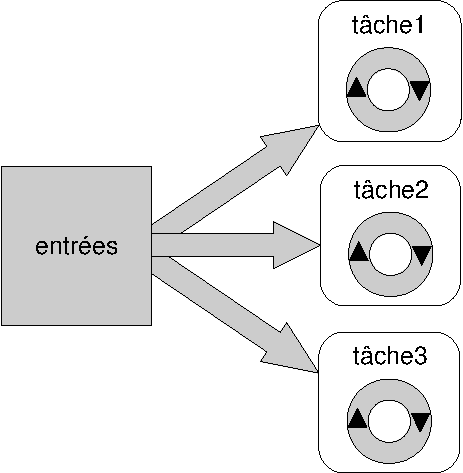
\includegraphics[scale=0.7]{model-peer}
  \caption{\label{fig:model-peer}Modèle pair}
\end{figure}


Exemple:
\begin{mdframed}
\begin{lstlisting}
main() {
  pthread_create( ... tache1);
  pthread_create( ... tache2);
  ...
  signale aux threads qu'ils peuvent commencer à travailler
}

tache1() {
  attend le signal de commencement
  effectue le traitement, et synchronise avec les autres threads si nécessaire
}

tache2() {
  attend le signal de commencement
  effectue le traitement, et synchronise avec les autres threads si nécessaire
}
\end{lstlisting}
\end{mdframed}
\subsection{Modèle pipeline}

Le modèle \emph{pipeline} (Figure \ref{fig:model-pipeline}) est exploitable lorsque les conditions suivantes sont remplies:

\begin{itemize}
  \item L'application traite une longue chaîne d'entrée;
  \item le traitement à effectuer sur ces entrées peut être décomposé en sous-tâches (étages de pipeline) au travers desquelles chaque donnée d'entrée doit passer;
  \item chaque étage peut traiter une donnée différente à chaque instant.
\end{itemize}

\begin{figure}[ht]
  \centering
  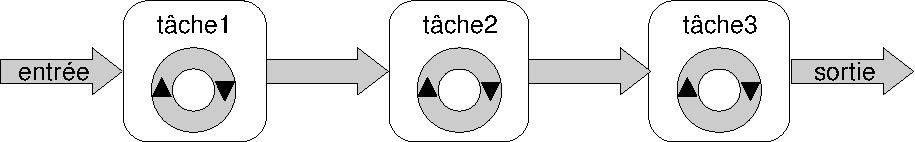
\includegraphics[scale=0.7]{model-pipeline}
  \caption{\label{fig:model-pipeline}Modèle pipeline}
\end{figure}


Là encore, un processeur multicœur devrait voir le temps d'exécution d'un programme grandement réduit. Un exemple typique permettant d'exploiter ce modèle serait du traitement sur un flux vidéo, où un étage modifierait la couleur, un autre le son, un autre appliquerait de la compression ...

Un étage du pipeline correspond donc à un traitement particulier à appliquer aux données. Le thread responsable de cet étage a un fonctionnement relativement simple. Il attend des données de l'étage précédent, traite ces données, et transmet ensuite le résultat de son traitement au thread responsable de l'étage suivant.
\newpage
Exemple:

\begin{lstlisting}
main() {
  pthread_create( ... etage1);
  pthread_create( ... etage2);
  ...
}

etage1() {
  boucle infinie {
    récupérer une entrée du programme
    traiter cette donnée
    passer le résultat à l'étage suivant
  }
}

etage2() {
  boucle infinie {
    récupérer une donnée de l'étage précédent
    traiter cette donnée
    passer le résultat à l'étage suivant
  }
}

etageN() {
  boucle infinie {
    récupérer une donnée de l'étage précédent
    traiter cette donnée
    passer le résultat en sortie du programme
  }
}
\end{lstlisting}

\chapter{Exclusion mutuelle}
\startchapter

\lettrine[lines=4]{L}{orsque} des tâches entrent en conflit pour l'accès à une ressource unique et non partageable, il devient nécessaire de limiter l'accès à la ressource à une seule tâche au plus et à chaque instant.  La ressource, qui ne peut être utilisée que par une seule tâche à la fois, peut être un périphérique ou une variable mise à jour par plusieurs tâches. Cette ressource, physique ou logique, est appelée {\em ressource critique}. Lorsqu'il s'agit de réaliser l'exclusion mutuelle entre des tâches dans un fragment de leur code, on appelle ces fragments des {\em sections critiques} plutôt que des ressources critiques. Remarquons que l'accès à un périphérique se fait aussi par un fragment de code.
\par
Illustrons le problème de l'exclusion mutuelle par un exemple.  Soient deux tâches $T_1$ et $T_2$ qui incrémentent une variable partagée $x$, initialisée à $0$.  Il est parfaitement raisonnable que la valeur finale après l'exécution de $T_1$ et de $T_2$ soit 1 ou 2.
Ceci est lié au fait que l'énoncé d'affectation n'est pas toujours implémenté comme une opération indivisible.  En effet, cet énoncé peut se traduire en 3 instructions assembleurs
\begin{displaymath}
\begin{array}{ccll}
       &                             & (1) & x \rightarrow \mbox{registre} \\
x:=x+1 & \Rightarrow & (2) & \mbox{inc registre} \\
       &                             & (3) & \mbox{registre} \rightarrow x
\end{array}
\end{displaymath}
Sous sa forme en assembleur, l'énoncé d'affectation peut être interrompu à deux endroits avant de compléter son exécution.  Pour résoudre le problème, il faut ordonner l'utilisation de la ressource critique.  Ainsi, si une tâche $T_i$ utilise la ressource et si une autre tâche $T_j$ désire elle aussi l'utiliser, alors $T_j$ doit
être retardée tant que $T_i$ ne la libère pas.
\noindent
Avant d'apporter une solution au problème de l'exclusion mutuelle, regardons quelques embûches à éviter.
\begin{enumerate}
\item {\em Il ne doit pas y avoir d'interblocage}.  La ressource critique doit être accessible.
\item {\em Il faut éviter la famine}.  Considérons la situation décrite à la figure~\ref{figex:famine} illustrant une ressource partagée entre 3 tâches.
 Si la situation représentée persiste, c.-à-d. que $T_1$ et $T_3$ utilisent à nouveau abondamment la ressource, $T_2$ n'accédera jamais à ressource et restera indéfiniment retardée.
\end{enumerate}

\begin{figure}[tb]
	\begin{center}
		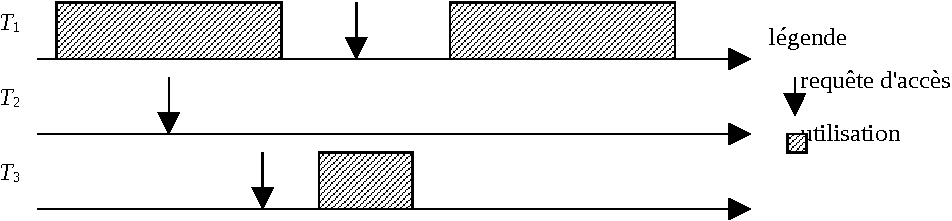
\includegraphics[width=.9\textwidth]{FigFamine}
		\caption{\label{figex:famine}Situation de famine}
	\end{center}
\end{figure}

\section{Classification des solutions}
Les différentes solutions apportées au problème de l'exclusion mutuelle que nous verrons peuvent être classées selon l'attente des tâches pour la ressource et selon l'environnement sur lequel ces tâches s'exécutent.
\par
L'attente des tâches à une ressource critique peut se caractériser suivant l'ordre dans lequel les tâches accèdent à la ressource.
\begin{itemize}
\item[(a)] L'attente est {\em PAPS} (FIFO en anglais) lorsque les tâches l'accèdent selon leur ordre d'arrivée.
\item[(b)] L'attente est {\em linéaire} lorsqu'une tâche ne peut accéder deux fois la ressource alors qu'une autre tâche est en attente.
Une tâche qui a obtenu la ressource et qui la redemande ne peut pas dépasser une tâche qu'elle a trouvé en attente auparavant.
\item[(c)] L'attente est {\em bornée par une fonction} $f(n)$ où $n$ est le nombre de tâches participantes à l'exclusion mutuelle, si une tâche désireuse d'accéder à la ressource ne peut pas se laisser dépasser que par un maximum de $f(n)$ tâches.
\item[(d)] L'attente est {\em finie} si elle n'est pas bornée mais pas infinie. Une tâche atteindra la ressource après un temps fini.  Il n'y a donc pas de famine.
\end{itemize}
\par
L'environnement joue un rôle dans la façon de résoudre le problème de l'exclusion mutuelle.  Ainsi nous distinguons les solutions {\em centralisées} et les solutions {\em réparties}. On appelle une solution centralisée, une solution qui repose sur l'existence d'une mémoire centrale pouvant être accédée par toutes les tâches en lecture ou en écriture. On appelle une solution répartie, une solution où il n'y a plus de mémoire commune.
Dans ce dernier cas, chaque tâche possède une mémoire locale dans laquelle elle est la seule à pouvoir lire et écrire. Les tâches peuvent s'échanger des résultats uniquement par le biais de messages. Il se peut donc que lorsqu'une tâche obtient la valeur d'une variable que cette valeur ait été modifiée entre temps. {\em Il y a pas de perception d'un état global en répartie.}
Dans ce qui suit on s'intéresse à plusieurs solutions possibles afin de résoudre le problème de l'exclusion mutuelle dans un environnement centralisé. L'exclusion mutuelle en répartie sera traitée dans l'unité d'enseignement {\em Programmation répartie.}

\section{Solutions logicielles par attente active}
Quoiqu'il existe des solutions matérielles au problème de l'exclusion mutuelle ou encore des solutions fournies par le noyau du système d'exploitation sur lequel repose nos tâches, l'étude de solutions logicielles présente deux facettes intéressantes.  L'une des difficultés rencontrée en traitement parallèle est notre intuition inadéquate pour confronter les opérations parallèles et pour saisir leur interaction. Une raison importante d'aborder ces solutions logicielles est donc d'élucider, par le biais d'arguments plutôt détaillés, les notions d'exécution atomique et d'attente bornée.
Les descriptions des relations temporelles et du comportement du logiciel s'avèreront suffisantes pour montrer rigoureusement, et ceci sans introduire d'outil mathématique nouveau, les propriétés des algorithmes.

Les solutions apportées au problème de l'exclusion mutuelle doivent satisfaire les contraintes suivantes.
\begin{enumerate}
\item On ne fait aucune hypothèse à propos des instructions ni du nombre de processeurs dans l'environnement.
On suppose uniquement que les instructions assembleurs (telles que load, store, etc.) sont exécutées atomiquement.  Si deux de ces instructions sont exécutées simultanément, le résultat sera le même que si elles étaient exécutées l'une après l'autre dans un ordre inconnu à priori.
\item On ne fait aucune hypothèse sur les vitesses relatives des tâches.
\item Lorsqu'une tâche n'est pas dans sa section critique, elle ne doit pas empêcher les autres tâches d'entrer dans leur section critique.
\item On ne doit pas remettre indéfiniment la décision qui consiste à admettre l'une des tâche qui est en compétition pour l'accès à la section critique.
\end{enumerate}
\par
Nous nous attardons maintenant à présenter les premiers algorithmes pour assurer l'exclusion mutuelle.  Ces algorithmes sont basés sur le principe de {\em l'attente active}.  Une tâche peut boucler sur une condition et l'évaluer de manière répétitive jusqu'à ce qu'elle change d'état.
\par
Dans le cadre de ce cours, nous nous limitons aux algorithmes qui synchronisent seulement deux tâches.  La généralisation de ces algorithmes à $n$ tâches ne fait pas partie du cours.  La présentation de ces algorithmes suit le schéma donné sur la figure~\ref{algex:générale}.
Les parties {\em prélude} et {\em postlude} constituent le protocole que doivent suivre les deux tâches \ccode{T0} et \ccode{T1} pour respectivement pénétrer et sortir de leur section critique.  Les parties des tâches non comprises entre les parties prélude et postlude constituent la partie non-critique.

\begin{figure}[!ht]

\begin{center}
\begin{tabular}{l}
\lstset{language=C++}
\begin{lstlisting}
// variables globales
void *T0(void *arg)
{
	while (true) {
		<prélude>
		<section critique>
		<postlude>
		<section non-critique>
	}
}

void *T1(void *arg)
{
	while (true) {
		<prélude>
		<section critique>
		<postlude>
		<section non-critique>
	}
}
\end{lstlisting}
\end{tabular}
\caption{\label{algex:générale}Schéma général des algorithmes d'exclusion mutuelle}
\end{center}
\end{figure}

\subsection*{Première tentative}
Le principe de la solution présentée sur l'algorithme~\ref{algex:tentative1} repose sur une variable booléenne appelée $occupe$ qui indique si l'une des tâches s'exécute en section critique.
Initialement, $occupe$ est positionné à faux.

\begin{algorithm}[!ht]
\caption{Première tentative d'exclusion mutuelle}\label{algex:tentative1}
\begin{center}
\begin{tabular}{l}
\lstset{language=C++}
\begin{lstlisting}
bool occupe = false;

void *T0(void *arg)
{
	while (true) {
		while (occupe)
			;
		occupe = true;
		/* section critique */
		occupe = false;
		/* section non-critique */
	}
}

void *T1(void *arg)
{
	while (true) {
		while (occupe)
			;
		occupe = true;
		/* section critique */
		occupe = false;
		/* section non-critique */
	}
}
\end{lstlisting}
\end{tabular}
\end{center}
\end{algorithm}

Malheureusement notre solution est incorrecte car on peut imaginer le scénario suivant.
\begin{center}
\begin{tabular}{cl}
$T_0$& lit $occupe$ à faux \\
$T_1$& lit aussi $occupe$ à faux \\
$T_1$& met $occupe$ à vrai \\
$T_1$& entre en section critique \\
$T_0$& met aussi $occupe$ à vrai \\
$T_0$& entre aussi en section critique. \\
\end{tabular}
\end{center}
Les deux tâches peuvent se retrouver simultanément en section critique.  Il n'y a donc pas d'exclusion mutuelle.

\subsection*{Deuxième tentative}
Notre deuxième tentative, algorithme ~\ref{algex:tentative2}, utilise une variable entière $tour$ qui indique l'identité de la tâche qui a l'autorisation d'accéder à la section critique.
Ainsi $T_i$ peut accéder à la section critique seulement si $tour$ est égale à $i$.

\begin{algorithm}[!ht]
\caption{Deuxième tentative d'exclusion mutuelle}\label{algex:tentative2}
\begin{center}
\begin{tabular}{l}
\lstset{language=C++}
\begin{lstlisting}
int tour = 0;  // ou 1

void *T0(void *arg)
{
	while (true) {
		while (tour != 0)
			;
		/* section critique */
		tour = 1;
		/* section non-critique */
	}
}

void *T1(void *arg)
{
	while (true) {
		while (tour != 1)
			;
		/* section critique */
		tour = 0;
		/* section non-critique */
	}
}
\end{lstlisting}
\end{tabular}
\end{center}
\end{algorithm}

Notre solution garantit qu'une seule tâche peut se trouver en section critique.  Cependant elle ne satisfait pas notre troisième contrainte.
Les tâches doivent exécuter leur section critique en alternance.
Une tâche peut donc attendre pour pénétrer en section critique alors que celle auquel le tour lui revient ne l'utilise pas et n'a peut-être plus l'intention de l'utiliser.
La plus lente des deux tâches impose son rythme à l'autre.  De plus, si une des deux tâches disparaît, l'autre attendra indéfiniment.

\subsection*{Troisième tentative}
Le problème avec notre solution précédente est lié au fait qu'elle tient compte de l'identité de la tâche qui peut accéder à la section critique sans considérer son état.
Pour remédier au problème, remplaçons la variable $tour$ de notre solution précédente par un vecteur de booléen $etat$ initialisé à faux.
Ainsi $etat[i]$ est vrai si $T_i$ est en section critique.
Malheureusement notre nouvelle solution, algorithme~\ref{algex:tentative3}, ne garantit plus l'exclusion mutuelle comme le montre la séquence qui suit.
\par\noindent
\begin{center}
\begin{tabular}{l}
$T_0$ exécute sa boucle et trouve $etat[1]$ à faux \\
$T_1$ exécute sa boucle et trouve aussi $etat [0]$ à faux \\
$T_0$ met $etat[0]$ à vrai et entre en section critique \\
$T_1$ met $etat[1]$ à vrai et entre aussi en section critique. \\
\end{tabular}
\end{center}
\par\noindent
Notre solution dépend des vitesses relatives des tâches.

\begin{algorithm}[!ht]
\caption{Troisième tentative d'exclusion mutuelle}\label{algex:tentative3}
\begin{center}
\begin{tabular}{l}
\lstset{language=C++}
\begin{lstlisting}
bool etat[2] = {false,false};

void *T0(void *arg)
{
	while (true) {
		while (etat[1])
			;
		etat[0] = true;
		/* section critique */
		etat[0] = false;
		/* section non-critique */
	}
}

void *T1(void *arg)
{
	while (true) {
		while (etat[0])
			;
		etat[1] = true;
		/* section critique */
		etat[1] = false;
		/* section non-critique */
	}
}
\end{lstlisting}
\end{tabular}
\end{center}
\end{algorithm}

\subsection*{Quatrième tentative}
Le problème avec notre troisième tentative provient du fait que l'une des tâches peut vérifier l'état de l'autre avant que cette dernière ait l'opportunité de modifier son état.  Corrigeons ce problème en déplaçant l'énoncé d'affectation comme l'illustre l'algorithme~\ref{algex:tentative4}.
Ainsi $etat[i]$ est vrai si $T_i$ désire accéder à la section critique.
\begin{algorithm}[!ht]
\caption{Quatrième tentative d'exclusion mutuelle}\label{algex:tentative4}
\begin{center}
\begin{tabular}{l}
\lstset{language=C++}
\begin{lstlisting}
bool etat[2] = {false,false};

void *T0(void *arg)
{
	while (true) {
		etat[0] = true;
		while (etat[1])
			;
		/* section critique */
		etat[0] = false;
		/* section non-critique */
	}
}

void *T1(void *arg)
{
	while (true) {
		etat[1] = true;
		while (etat[0])
			;
		/* section critique */
		etat[1] = false;
		/* section non-critique */
	}
}
\end{lstlisting}
\end{tabular}
\end{center}
\end{algorithm}

L'exclusion mutuelle est à présent garantie mais un autre problème surgit.
Si $T_0$ met $etat[0]$ à vrai et juste après $T_1$ met $etat[1]$ à vrai, alors $T_0$ et $T_1$ bouclent indéfiniment.
Si les deux tâches progressent simultanément dans leur prélude elles se bloquent mutuellement.
Chacune croit que l'autre est engagée dans sa section critique.
Ceci provient du fait que $T_i$ indique son intention d'entrer en section critique sans connaître l'intention de l'autre.

\subsection*{Cinquième tentative}
Modifions notre précédente tentative de manière à obliger une tâche à renoncer temporairement à son désir de pénétrer en section critique si l'autre tâche désire elle aussi y entrer.
Cette nouvelle tentative est donnée par l'algorithme~\ref{algex:tentative5}.
\begin{algorithm}[!ht]
\caption{Cinquième tentative d'exclusion mutuelle}\label{algex:tentative5}
\begin{center}
\begin{tabular}{l}
\lstset{language=C++}
\begin{lstlisting}
bool etat[2] = {false,false};

void *T0(void *arg)
{
	while (true) {
		etat[0] = true;
		while (etat[1]) {
			etat[0] = false;
			while (etat[1])
				;
			etat[0] = true;
		}
		/* section critique */
		etat[0] = false;
		/* section non-critique */
	}
}

void *T1(void *arg)
{
	while (true) {
		etat[1] = true;
		while (etat[0]) {
			etat[1] = false;
			while (etat[0])
				;
			etat[1] = true;
		}
		/* section critique */
		etat[1] = false;
		/* section non-critique */
	}
}
\end{lstlisting}
\end{tabular}
\end{center}
\end{algorithm}

Bien que l'exclusion mutuelle soit garantie, un interblocage est possible si les deux tâches exécutent leur prélude en alternance.
\par\noindent
\begin{center}
\begin{tabular}{l}
$T_0$ met $etat[0]$ à vrai \\
$T_1$ met $etat[1]$ à vrai \\
$T_0$ exécute sa boucle externe et trouve $etat[1]$ à vrai \\
$T_1$ exécute sa boucle externe et trouve $etat[0]$ à vrai \\
$T_0$ met $etat[0]$ à faux  \\
$T_1$ met $etat[1]$ à faux \\
$T_0$ exécute sa boucle interne et trouve $etat[1]$ à faux \\
$T_1$ exécute sa boucle interne et trouve $etat[0]$ à faux \\
$T_0$ met $etat[0]$ à vrai \\
$T_1$ met $etat[1]$ à vrai \\
etc. \\
\end{tabular}
\end{center}
\par\noindent
Cette séquence d'instructions a très peu de chance de se produire en réalité. Elle nécessite en effet, des conditions difficiles à réaliser.

\section{Algorithme de Dekker}
On remarque qu'au fur et à mesure que nous progressons vers une solution, celle-ci se complique. L'algorithme de Dekker est une solution qui combine nos deuxième et cinquième tentatives.
L'algorithme~\ref{algex:Dekker} est basé sur notre dernière tentative mais règle le problème d'interblocage en donnant priorité à l'une des deux tâches.  La variable $tour$ de notre deuxième tentative impose l'ordre dans lequel les tâches accèdent à la section critique.  En cas de conflit, l'une des tâches se résigne temporairement pour donner l'accès à l'autre tâche.
\begin{algorithm}[!ht]
\caption{Algorithme de Dekker}\label{algex:Dekker}
\begin{center}
\begin{tabular}{l}
\lstset{language=C++}
\begin{lstlisting}
bool etat[2] = {false,false};
int tour = 0; // ou 1

void *T0(void *arg)
{
	while (true) {
		etat[0] = true;
		while (etat[1])
			if (tour == 1) {
				etat[0] = false;
				while (tour == 1)
					;
				etat[0] = true;
			}
		/* section critique */
		tour = 1;
		etat[0] = false;
		/* section non-critique */
	}
}

void *T1(void *arg)
{
	while (true) {
		etat[1] = true;
		while (etat[0])
			if (tour == 0) {
				etat[1] = false;
				while (tour == 0)
					;
				etat[1] = true;
			}
		/* section critique */
		tour = 0;
		etat[1] = false;
		/* section non-critique */
	}
}
\end{lstlisting}
\end{tabular}
\end{center}
\end{algorithm}

Montrons que l'algorithme de Dekker garantit l'exclusion mutuelle et ensuite qu'il n'y a pas d'interblocage possible.
\par
Pour montrer que l'exclusion mutuelle est préservée, supposons que $T_0$ et $T_1$ sont toutes les deux en section critique. Dans ce cas, $etat[i]$ = vrai pour $i=0$ et $1$.  Les deux tâches n'ont pas pu entrer en même temps car aucune n'aurait pu sortir de leur boucle externe.  Conséquemment l'une des tâches est entrée avant l'autre.  Soit $T_0$ cette tâche.
$T_0$ a alors trouvé $etat[1]$ à faux.  Comme seule $T_1$ peut modifier $etat[1]$ et comme $T_1$ ne vérifie $etat[0]$ que si $etat[1]$ est à vrai, il s'ensuit que $T_1$ est soit dans sa boucle interne ou soit dans sa partie non-critique.  Si $T_1$ se trouve dans sa boucle interne, elle n'en sortira que lorsque $T_0$ exécute son postlude.
Par contre si $T_1$ se trouve en section non-critique, elle bouclera dans son prélude si elle désire accéder à la section critique.  Un raisonnement analogue peut être fait dans le cas où $T_1$ entre en section critique avant $T_0$.
La propriété d'exclusion mutuelle est donc montrée.
\par
Montrons à présent que l'interblocage n'est pas possible.
Supposons d'abord le cas où seule une tâche désire entrer en section critique. Elle passe alors directement en section critique, peu importe la valeur de $tour$.  Admettons maintenant que les deux tâches veulent entrer en section critique, et que $tour$ vaut 0. Deux cas sont possibles. Si $T_0$ trouve $etat[1]$ à faux,
elle pénètre directement en section critique.
(Le raisonnement est identique pour $T_1$.)
Par contre, si $T_0$ trouve $etat[1]$ à vrai, $T_0$ attend dans sa boucle externe jusqu'à ce que $etat[1]$ passe à faux. Pendant ce temps, $T_1$ attend dans sa boucle interne jusqu'à ce que $tour$ soit égal à 1.  Mais auparavant, $T_1$ positionne $etat[1]$ à faux, ce qui permet à $T_0$ de sortir de sa boucle et de pénétrer en section critique. $T_0$ entre donc en section critique avant $T_1$ car la variable $tour$ lui donne avantage.  Si $tour$ valait 1, l'inverse se produit et $T_1$ pénètre avant $T_0$.  Il n'y a donc pas d'interblocage.
\par
Finalement, montrons que le risque de famine repose uniquement sur celui du matériel.  Une famine peut se produire lorsque $T_i$ trouve sans cesse $etat[j]$ à faux et pénètre en section critique alors que $T_j$ est incapable de mettre $etat[j]$ à vrai empêché par les lectures répétitives de cette variable par $T_i$.
L'algorithme se fie sur le matériel pour l'équité des requêtes mémoires.  L'algorithme résout donc les conflits en un temps fini.

\section{Algorithme de Peterson}
Avant de conclure, nous présentons un dernier algorithme, algorithme~\ref{algex:Peterson}, qui est remarquable par sa simplicité.
\begin{algorithm}[!ht]
\caption{Algorithme de Peterson}\label{algex:Peterson}
\begin{center}
\begin{tabular}{l}
\lstset{language=C++}
\begin{lstlisting}
bool intention[2] = {false,false};
int tour = 0; // ou 1

void *T0(void *arg)
{
	while (true) {
		intention[0] = true;
		tour = 1;
		while (intention[1] && tour == 1)
			;
		/* section critique */
		intention[0] = false;
		/* section non-critique */
	}
}

void *T1(void *arg)
{
	while (true) {
		intention[1] = true;
		tour = 0;
		while (intention[0] && tour == 0)
			;
		/* section critique */
		intention[1] = false;
		/* section non-critique */
	}
}
\end{lstlisting}
\end{tabular}
\end{center}
\end{algorithm}

Les variables partagées entre les deux tâches sont
\begin{center}
\begin{tabular}{l}
\lstset{language=C++}
\begin{lstlisting}
		bool intention[2] = {false,false};
		int tour = 0; // ou 1
\end{lstlisting}
\end{tabular}
\end{center}
\par\noindent
Lorsque la tâche $T_i$ veut accéder à la section critique, elle positionne $intention[i]$ à vrai.  La variable $tour$ départage les deux tâches si celles-ci désirent accéder en même temps à la section critique.
\par
Pour vérifier que l'exclusion mutuelle est conservée, supposons que $T_0$ et $T_1$ sont toutes les deux dans leurs sections critiques.
Dans ce cas, $intention[i]$ $=$ vrai pour $i = 0$ et 1.  Mais ces tâches n'ont pas pu sortir de leurs boucles en même temps car $tour$ ne peut prendre simultanément la valeur 0 et la valeur 1.  L'une des tâches est donc entrée en section critique avant l'autre. Supposons que c'est $T_i$. $T_i$ a alors évalué la condition de sa boucle pendant que $T_j$ exécutait $tour$ $=$ $i$.  Mais à ce moment, $T_j$ trouve $intention[i]$ à vrai et $tour$ à $i$ lorsqu'elle évalue la condition de sa boucle.
Cette condition sera évaluée à vrai car ces variables conservent leurs valeurs tant que $T_i$ se trouve en section critique, ce qui préserve l'exclusion mutuelle.
\par
Pour vérifier qu'il n'y a pas d'interblocage, remarquons qu'une tâche $T_i$ ne peut être bloquée dans son prélude que si elle trouve sans cesse $intention[j]=$vrai et $tour=j$.  Si $T_j$ ne désire pas accéder à la section critique, $intention[j]$ est à faux et $T_i$ ne peut pas être bloquée.  Par contre si $intention[j]$ est à vrai, $T_j$ doit aussi être dans sa boucle pour qu'il y ait interblocage.  Mais à ce moment, la variable $tour$, valant nécessairement 0 ou 1, favorisera l'une des deux tâche.  Il ne peut donc pas y avoir d'interblocage.
\par
Pour montrer que le protocole est équitable, il suffit de montrer que si $T_i$ est dans sa boucle d'attente et que $T_j$ est dans sa section critique, $T_i$ pénétrera en section critique avant $T_j$ si celle-ci désire à nouveau entrer en section critique.  Lorsque $T_j$ sort de son postlude, $intention[j]$ est à faux et $T_i$ peut accéder à son tour à la section critique.  Si $T_j$ désire à nouveau entrer en section critique, elle repositionne $intention[j]$ à vrai et $tour$ à $i$.  Ainsi $T_j$ est bloquée dans sa boucle d'attente tant que $T_i$ n'accède pas à la section critique.
\par
Les deux algorithmes, Dekker et Peterson, se généralisent à $n$ tâches. Toutefois, cette généralisation sort du cadre de ce cours.

\section{Exercices}

\startexercice

Soit les deux tâches $T_0$ et $T_1$ données sur la figure~\ref{algex:Exercice1} et devant réaliser l'exclusion mutuelle dans leur section critique.
\begin{figure}[!ht]

\begin{center}
\begin{tabular}{l}
\lstset{language=C++}
\begin{lstlisting}
bool intention[2] = {false,false};
int tour = 0; // ou 1

void *T0(void *arg)
{
	while (true) {
		intention[0] = true;
		while (tour != 0) {
			while (intention[1])
				;
			tour = 0;
		}
		/* section critique */
		intention[0] = false;
		/* section non-critique */
	}
}

void *T1(void *arg)
{
	while (true) {
		intention[1] = true;
		while (tour != 1) {
			while (intention[0])
				;
			tour = 1;
		}
		/* section critique */
		intention[1] = false;
		/* section non-critique */
	}
}
\end{lstlisting}
\end{tabular}
\caption{\label{algex:Exercice1}Exercice 1}
\end{center}
\end{figure}
L'exclusion mutuelle est-elle garantie par les parties prélude et postlude des tâches? Justifiez votre réponse.

\chapter{Verrous et sémaphores}
\startchapter

\lettrine[lines=4]{L}{es} solutions au problème de l'exclusion mutuelle présentées jusqu'à présent sont difficiles à réaliser et à comprendre car il n'est jamais clair si une variable est utilisée pour implémenter l'exclusion mutuelle où si elle est utilisée pour autre chose.
De plus ces solutions sont basées sur l'attente active~:  une tâche qui ne peut pas progresser dans sa partie prélude occupe inutilement le processeur.  Un processeur peut être utilisé d'une façon plus productive s'il n'attend pas activement qu'une condition change d'état.

\section{Verrou}\label{verrou:intro}
Les {\em verrous} ont été introduits pour résoudre (partiellement) ces problèmes. Un verrou $v$ est une variable booléenne sur laquelle deux opérations atomiques sont définies, $Verrouille(v)$ et $D\acute{e}verrouille(v)$.  Ce sont les deux seules opérations (mis à part la création et sa destruction) qui peuvent manipuler le verrou.
Les primitives $Verrouille(v)$ et $D\acute{e}verrouille(v)$ sont équivalentes à l'exécution atomique des séquences d'instructions données ci-dessous.

\begin{center}
\begin{tabular}{l}
\lstset{language=C++}
\begin{lstlisting}
void Verrouille(verrou v)
{
	if (v)
		v = false;
	else
		suspendre la tâche appelante dans la file associée à v
}

void Déverrouille(verrou v)
{
	if (la file associée à v != vide)
		débloquer une tâche en attente dans file
	else
		v = true;
}
\end{lstlisting}
\end{tabular}
\end{center}
\par
Ainsi, si un verrou $v$ est initialisé à vrai et qu'une tâche appelle $Verrouille(v)$, le verrou est positionné à faux. Si une seconde tâche appelle $Verrouille(v)$, alors cette tâche, qui est à l'état élu, passe à l'état bloqué et joint la file d'attente associée à $v$.
La primitive $D\acute{e}verrouille(v)$ réalise l'opération inverse. S'il y a une tâche en attente sur le verrou $v$, alors cette tâche est réactivée. La tâche réveillée sort de la file d'attente associée à $v$ pour joindre la file des tâches prêtes. Remarquons que l'exécution de la primitive $D\acute{e}verrouille(v)$ revient à passer le verrou $v$ à la tâche réveillée.
S'il n'y a pas de tâche en attente pour obtenir le verrou $v$, la primitive $D\acute{e}verrouille(v)$ libère le verrou $v$ en le positionnant à vrai (état initial).

\subsection{Section critique}
Comme son nom le sous-entend, un verrou permet de résoudre le problème de l'exclusion mutuelle à $n$ tâches de manière simple. Il suffit de verrouiller un verrou $v$ avant d'entrer en section, bloquant ainsi les autres tâches qui accèdent à leur section critique protégée par le même verrou $v$. La sortie d'une section critique se fait en déverrouillant $v$, ce qui libère le verrou ou réveille une tâche bloquée pour l'accès à sa section critique.
\begin{center}
\vspace{-0.2 cm}
\begin{tabular}{l}
\hspace{0.6 cm}$\vdots$ \\
\begin{lstlisting}
Verrouille(v);
/* section critique */
Déverrouille(v);
\end{lstlisting} \\
\hspace{0.6 cm}$\vdots$
\end{tabular}
\end{center}

\subsection{Verrous en Posix}
Mis à part de définir un ensemble de fonctions permettant de gérer des threads, la bibliothèque Pthread contient aussi des fonctions manipulant des verrous.
Ces verrous sont prévus pour résoudre le problème de l'exclusion mutuelle. C'est pourquoi les noms de ces fonctions sont préfixés par \ccode{pthread_mutex}, où {\em mutex} est l'abréviation anglaise de {\em mutual exclusion}. Une description complète de ces fonctions est fournie à l'annexe A des notes de cours.

Il y a 2 façons pour créer un verrou. La première, et la plus simple, consiste à définir une variable globale de type \ccode{pthread_mutex_t} et de l'initialiser par le symbole \ccode{PTHREAD_MUTEX_INITIALIZER}. La seconde façon consiste à initialiser le verrou par la fonction \ccode{pthread_mutex_init()}. Cette méthode est indiquée si le verrou est créé dynamiquement, c.-à-d. quand une variable de type \ccode{pthread_mutex_t} est allouée par \ccode{malloc()}. Ces initialisations préparent le verrou pour réaliser la protection d'une section critique.

Les 2 opérations de verrouillage et de déverrouillage du verrou deviennent en Pthread des appels aux fonctions \ccode{pthread_mutex_lock} et \ccode{pthread_mutex_unlock} respectivement. Ces 2 fonctions ont exactement la sémantique des primitives que nous avons vu à la section \ref{verrou:intro}.

Il y a une troisième primitive, \ccode{pthread_mutex_trylock}, qui est un verrouillage immédiat. Si, au moment de l'appel, le verrou est déjà verrouillé, la fonction ne bloque pas l'appelant mais retourne la valeur \ccode{EBUSY}. Une tâche peut donc essayer de s'emparer d'un verrou, et si celui-ci est déjà pris, de faire autre chose.
\begin{center}
\vspace{-0.2 cm}
\begin{tabular}{l}
\begin{lstlisting}
switch (pthread_mutex_trylock(&verrou)) {
	case 0: printf("%d prend le verrou\n",threadID); break;
	case EBUSY: printf("Le verrou est pris par un autre thread\n"); break;
	case EINVAL: printf("Le verrou est invalide\n");
  default: break;
}
\end{lstlisting}
\end{tabular}
\end{center}

Généralement un verrou a une existence équivalente à celle du thread principal. Mais il y a des situations où un verrou est créé pour accomplir une action précise et cesse d'être utile par la suite. Pour ce cas, Pthread met à disposition une fonction permettant de libérer toutes les ressources associées au verrou. Cette fonction s'appelle \ccode{pthread_mutex_destroy}.

\subsection{Coordination de tâches}
Les verrous peuvent aussi servir à résoudre les problèmes liés à la coordination (ou synchronisation) de tâches.  Par exemple, si deux tâches $T1$ et $T2$ exécutent respectivement les instructions $I_1$ et $I_2$, et que $I_1$ doit précéder l'exécution de $I_2$, la synchronisation se réalise avec un verrou $sync$ initialisé à son état verrouillé.
L'algorithme \ref{verrou:synchro1} illustre l'exemple.

\begin{algorithm}[!ht]
\caption{Coordination de 2 tâches par un verrou}\label{verrou:synchro1}
\begin{center}
\begin{tabular}{l}
\begin{lstlisting}
#include <pthread.h>
#include <stdio.h>
#include <stdlib.h>

static pthread_mutex_t sync = PTHREAD_MUTEX_INITIALIZER;

void *T1(void *arg) {
  sleep(1);                                    // I_1
  printf("T1: fini sleep\n");
  pthread_mutex_unlock(&sync);
  return NULL;
} /* fin de T1 */

void *T2(void *arg) {
  printf("T2: avant pthread_mutex_lock\n");
  pthread_mutex_lock(&sync);
  printf("T2: apres pthread_mutex_lock\n");   // I_2
  return NULL;
} /* fin de T2 */

int main(void) {
  pthread_t tache1, tache2;
  pthread_mutex_lock(&sync);
  if (pthread_create(&tache1,NULL,T1,NULL) == 0) {
     if (pthread_create(&tache2,NULL,T2, NULL) == 0) {
        pthread_join(tache1,NULL);
        pthread_join(tache2,NULL);
        return EXIT_SUCCESS;
     }
  }
  return EXIT_FAILURE;
} /* fin de main */
\end{lstlisting}
\end{tabular}
\end{center}
\end{algorithm}

Remarquons que le verrou $sync$ est initialisé pour une exclusion mutuelle et, avant de lancer l'exécution des tâches \ccode{T1} et \ccode{T2}, le verrou $sync$ est verrouillé. Ainsi, si \ccode{T2} est plus rapide que \ccode{T1}, \ccode{T2} se bloque jusqu'à ce que \ccode{T1} relâche le verrou pris par \ccode{main}.

On peut généraliser le problème précédent pour que deux tâches se synchronisent de la manière suivante. Chaque tâche dispose d'une activité qu'elle peut exécuter, suivie d'une autre activité pouvant être démarrée quand l'autre tâche a terminé sa première activité.
Schématiquement, nous avons
\begin{center}
\vspace{-0.2 cm}
\begin{tabular}{lccc}
&{\em TâcheA} & \hspace{0.5 cm} & {\em TâcheB} \\
Premières activités &\ccode{a1}     &  & \ccode{b1} \\
Rendez-vous & & $\times$ & \\
Deuxièmes activités &\ccode{a2}     &  & \ccode{b2}
\end{tabular}
%\begin{tabular}{ccc}
%{\em TâcheA} & \hspace{0.5 cm} & {\em TâcheB} \\
%\ccode{a1}     &  & \ccode{b1} \\
%\ccode{a2}     &  & \ccode{b2}
%\end{tabular}
\end{center}

Les activités \ccode{a2} et \ccode{b2} ne peuvent débuter que lorsque les activités \ccode{a1} et \ccode {b1} ont terminés. Ce type de synchronisation s'appelle {\em rendez-vous}. Les 2 tâches ont un point de rencontre où aucune ne peut continuer avant que l'autre n'arrive à ce point.

\subsubsection*{Première solution}
\begin{algorithm}[t]
\caption{Première solution: Rendez-vous entre 2 tâches}\label{verrou:synchro2}
\begin{center}
\begin{tabular}{l}
\begin{lstlisting}
#include <pthread.h>
#include <stdio.h>
#include <stdlib.h>

static pthread_mutex_t arriveA = PTHREAD_MUTEX_INITIALIZER;
static pthread_mutex_t arriveB = PTHREAD_MUTEX_INITIALIZER;

void *TacheA(void *arg) {
  a1;
  pthread_mutex_lock(&arriveB);
  pthread_mutex_unlock(&arriveA);
  a2;
  return NULL;
} /* fin de TacheA */

void *TacheB(void *arg) {
  b1;
  pthread_mutex_unlock(&arriveB);
  pthread_mutex_lock(&arriveA);
  b2;
  return NULL;
} /* fin de TacheB */

int main(void) {
  pthread_t tacheA, tacheB;
  pthread_mutex_lock(&arriveA);
  pthread_mutex_lock(&arriveB);
  if (pthread_create(&tacheA,NULL,TacheA,NULL) == 0) {
     if (pthread_create(&tacheB,NULL,TacheB,NULL) == 0) {
        pthread_join(tacheA,NULL);
        pthread_join(tacheB,NULL);
        return EXIT_SUCCESS;
     }
  }
  return EXIT_FAILURE;
} /* fin de main */
\end{lstlisting}
\end{tabular}
\end{center}
\end{algorithm}

Notre première solution (algorithme \ref{verrou:synchro2}) demande un nombre élevé de changements de contexte. En effet, sur un monoprocesseur ou pour une exécution asynchrone, l'une des tâches arrivera au point de rendez-vous avant l'autre. Si \ccode{TacheA} arrive la première, la tâche se bloquera sur le verrou \ccode{arriveB}, puis lorsque \ccode{TacheB} termine \ccode{b1}, \ccode{TacheB} déverrouille \ccode{arriveB} avant de se bloquer sur \ccode{arriveA}. La tâche \ccode{TacheA} peut alors reprendre son exécution et déverrouiller \ccode{arriveA} avant de progresser à son activité \ccode{a2}. Dans ce cas, il y a 3 changements de contexte. Si, au contraire \ccode{TacheB} termine \ccode{b1} et arrive au point de rendez-vous avant \ccode{TacheA}, le fait de déverrouiller \ccode{arriveB} puis attendre sur \ccode{arriveA}, permet à \ccode{TacheA} de terminer son activité \ccode{a1}, puis de poursuive à \ccode{a2} sans changement de contexte.

\subsubsection*{Deuxième solution}
\begin{algorithm}[t]
\caption{Deuxième solution: rendez-vous entre 2 tâches}\label{verrou:synchro3}
\begin{center}
\begin{tabular}{l}
\begin{lstlisting}
...
void *TacheA(void *arg) {
  a1;
  pthread_mutex_unlock(&arriveA);
  pthread_mutex_lock(&arriveB);
  a2;
  return NULL;
} /* fin de TacheA */

void *TacheB(void *arg) {
  b1;
  pthread_mutex_unlock(&arriveB);
  pthread_mutex_lock(&arriveA);
  b2;
  return NULL;
} /* fin de TacheB */
...
\end{lstlisting}
\end{tabular}
\end{center}
\end{algorithm}
Notre seconde solution, donnée sur algorithme \ref{verrou:synchro3}, minimise le nombre de changements de contexte. Ici, la dernière tâche qui arrive au point de rendez-vous informe l'autre via un déverrouillage, puis peut prendre le verrou positionné par l'autre tâche avant de poursuive. C'est uniquement la première tâche qui atteint le rendez-vous qui devra subir un changement de contexte.

\section{Sémaphores}
Les {\em sémaphores} sont une généralisation des verrous. Un sémaphore $s$ est une variable entière sur laquelle deux opérations atomiques sont définies, $P(s)$ (pour tester: Proberen) et $V(s)$ (pour incrémenter: Verhogen). Comme pour un verrou, ce sont les deux seules opérations (mis à part la création et l'initialisation) qui peuvent manipuler le sémaphore. Ainsi, un sémaphore généralise les valeurs que peuvent prendre le verrou, c'est la raison pour laquelle les verrous sont souvent appelés des {\em sémaphores binaires}, car ils sont limités à 2 valeurs.
Les primitives $P(s)$ et $V(s)$ sont équivalentes à l'exécution atomique des séquences d'instructions données ci-dessous.

\begin{center}
\begin{tabular}{l}
\begin{lstlisting}
void P(sémaphore s)
{
	s -= 1;
	if (s < 0)
		suspendre la tâche appelante dans la file associée à s
}

void V(sémaphore s)
{
	s += 1;
	if (s <= 0)
		débloquer une des tâches de la file associée à s
}
\end{lstlisting}
\end{tabular}
\end{center}
\par
Avant de voir comment implémenter ces opérations, regardons d'abord quelques problèmes simples résolus par les sémaphores.
Les sémaphores peuvent résoudre l'exclusion mutuelle avec $n$ tâches pouvant accéder à la ressource.
Les tâches se partagent un sémaphore $mutex$ initialisé à 1.  Le protocole pour chaque tâche devient tout simplement
\begin{center}
\begin{tabular}{l}
\hspace{0.6 cm}$\vdots$ \\
\begin{lstlisting}
P(mutex);
/* section critique */
V(mutex);
\end{lstlisting} \\
\hspace{0.6 cm}$\vdots$
\end{tabular}
\end{center}
\par
Selon la valeur $v>0$ à laquelle est initialisée \ccode{mutex}, jusqu'à $v$ tâches peuvent être admises simultanément dans la section critique.  On parle dans cas de {\em section contrôlée} plutôt que de section critique.  L'exclusion mutuelle devient un cas particulier d'un problème plus général~:  limiter à $n$ le nombre de tâches pouvant se trouver ensemble dans une section.

Les sémaphores servent aussi à résoudre les problèmes liés à la coordination (ou synchronisation) de tâches.  Par exemple, si deux tâches $T_1$ et $T_2$ exécutent respectivement les instructions $I_1$ et $I_2$, et que $I_1$ doit précéder l'exécution de $I_2$, la synchronisation se réalise avec un sémaphore $sync$ initialisé à 0 comme
suit
\begin{center}
\begin{tabular}{l}
\begin{lstlisting}
void *T1(void *arg)
{
	...
	I1;
	V(sync);
	...
}
\end{lstlisting}
\hspace{1 cm}
\begin{lstlisting}
void *T2(void *arg)
{
	...
	P(sync);
	I2;
	...
}
\end{lstlisting}
\end{tabular}
\end{center}

\section{Implémentation des sémaphores}
Nous avons vu qu'une file d'attente est associée à chaque sémaphore. Cette file contient toutes les tâches bloquées sur ce sémaphore.  Un sémaphore peut donc se définir de la façon suivante
\begin{center}
\begin{tabular}{l}
\begin{lstlisting}
typedef struct {
	unsigned int valeur;
	DescripteurDeTâche *liste;
} sémaphore;
\end{lstlisting}
\end{tabular}
\end{center}
Lorsqu'une tâche se bloque sur un sémaphore, elle est ajoutée à la liste des tâches de ce sémaphore. Lors de l'opération $V$, une des tâches est enlevée de la liste, puis réactivée. Ceci consiste à changer l'état de tâche à {\em prêt}, puis de l'insérer dans la file des tâches éligibles pour le processeur. La file d'attente d'un sémaphore s'implémente facilement avec une liste chaînée de descripteurs de processus. Le sémaphore contient un pointeur vers la liste de descripteurs.  Chaque descripteur contient aussi un pointeur pour assurer la continuité de la liste. La gestion des insertions et des retraits est l'aspect qui rend le sémaphore équitable ou non.  La gestion peut se faire comme une pile, toutefois il y aura un risque évident de famine.  La solution la plus courante est évidemment de l'implémenter comme une file PAPS.  On pourrait envisager des priorités ou n'importe quelle discipline de service.
\par
Il est intéressant d'observer l'implémentation telle que proposée, qui utilise une valeur de sémaphore non signée. Le passage dans les valeurs négatives, qui serait observé avec la réalisation de $P$ et $V$ telle que précédemment illustrée est en fait réalisée en laissant la valeur à 0, et en comptant le nombre de threads en attente dans la liste.
\par
Nous pouvons noter que l'implémentation des verrous est très similaire à celle des sémaphores, si ce n'est que la valeur entière est remplacée par un booléen. Le reste du fonctionnement, en ce qui concerne la liste en attente, est identique.
\par
Pour garantir l'atomicité des primitives $P$ et $V$, les méthodes diffèrent selon l'architecture de l'ordinateur.
Sur une machine monoprocesseur, il suffit d'inhiber les interruptions pour interdire les commutations de tâches.  Remarquons que le problème de l'exclusion mutuelle peut aussi se résoudre en inhibant les interruptions avant d'accéder en section critique, et en permettant à nouveau les interruptions en sortant de la section critique.
Il est toutefois fortement déconseillé d'assurer l'exclusion mutuelle à l'aide d'une des solutions logicielles (attente active) que nous avons étudiées au chapitre 2.

\section{Equivalence entre verrous et sémaphores}
En apparence, un sémaphore semble plus puissant qu'un verrou. Mais que faire si la plateforme à disposition ne possède que des verrous? Il faut dans ce cas réaliser ou simuler un sémaphore en n'utilisant que des verrous. La méthode est donnée par l'algorithme \ref{semaex:verrou}. Le verrou \ccode{mutex} protège la structure partagée \ccode{Semaphore} et le verrou \ccode{attente} simule la file d'attente du sémaphore.
Les verrous sont donc aussi généraux que les sémaphores; autrement dit, il n'existe aucun problème pouvant être résolu par un sémaphore et pour lequel il n'y a pas de solution en n'utilisant que des verrous.
\begin{algorithm}
\caption{Implémentation de sémaphores par verrous}\label{semaex:verrou}
\lstset{language=C++}
\begin{lstlisting}
typedef struct {
    pthread_mutex_t mutex, attente;
    int valeur;
} Semaphore;

Semaphore *CreerSemaphore(unsigned val) {
    Semaphore *s = (Semaphore *)malloc(sizeof(Semaphore));
    if (s != NULL) {
        pthread_mutex_init(&s->mutex,NULL);
        pthread_mutex_init(&s->attente,NULL);
        pthread_mutex_lock(&s->attente);
        s->valeur = val;
    }
    return s;
}

void P(Semaphore *s) {
    pthread_mutex_lock(&s->mutex);
    s->valeur -= 1;
    if (s->valeur < 0) {
        pthread_mutex_unlock(&s->mutex);
        pthread_mutex_lock(&s->attente);
    }
    pthread_mutex_unlock(&s->mutex);
}

void V(Semaphore *s) {
    pthread_mutex_lock(&s->mutex);
    s->valeur += 1;
    if (s->valeur <= 0)
        pthread_mutex_unlock(&s->attente);
    else
        pthread_mutex_unlock(&s->mutex);
}

void DetruireSemaphore(Semaphore *s) {
    pthread_mutex_destroy(&s->mutex);
    pthread_mutex_destroy(&s->attente);
    free(s);
}
\end{lstlisting}
\end{algorithm}

%\subsection{Sémaphores Posix}

%... à faire.

\section{Exercices}

\startexercice

Comment faut-il modifier l'implémentation d'un sémaphore donnée par l'algorithme \ref{semaex:verrou} si nous voulons que les valeurs du sémaphore soient sur des entiers non signés (\ccode{unsigned int})?

\startexercice

Comment implémentez-vous un verrou si vous ne disposez que de sémaphores? La sémantique du verrou doit évidemment être préservée.

% non distribué aux étudiants

\startexercice

Commentez la différence entre les deux codes suivants:

\begin{lstlisting}
void *tache(void *) {
  pthread_mutex_t mutex=PTHREAD_MUTEX_INITIALIZER;
  pthread_mutex_lock(&mutex);
  printf("Section critique\n");
  pthread_mutex_unlock(&mutex);
}
\end{lstlisting}

\begin{lstlisting}
void *tache(void *) {
  static pthread_mutex_t mutex=PTHREAD_MUTEX_INITIALIZER;
  pthread_mutex_lock(&mutex);
  printf("Section critique\n");
  pthread_mutex_unlock(&mutex);
}
\end{lstlisting}

\startexercice

Nous désirons réaliser une application possédant 2 tâches. Le programme principal est en charge de lancer les deux tâches.

Etant donné que les tâches, une fois lancées, doivent attendre un signal du programme principal pour s'exécuter, comment résoudre le problème à l'aide de verrous?

Et à l'aide de sémaphores?

\chapter{Producteurs-consommateurs}
\startchapter
\section{Enoncé du problème}
Une tâche productrice place des éléments dans un tampon pour qu'une tâche consommatrice puisse les retirer et les traiter. Le tampon peut contenir un nombre maximum d'éléments et ces éléments sont organisés en liste circulaire. Un élément du tampon, dont le contenu a été consommé, peut à nouveau servir.

Ce schéma constitue une communication entre 2 tâches, la productrice étant l'émettrice du message et la consommatrice, la destinatrice du message. C'est aussi la seule manière de transférer des données contenues dans une tâche vers une autre tâche. Dans ce qui suit, nous généralisons le problème à un nombre quelconque de tâches. N'importe quelle productrice peut alors déposer un élément dans un tampon et aussi n'importe quelle consommatrice peut la retirer. Notons que la séparation des tâches en productrices et consommatrice n'est qu'à des fins d'exposition et pour distinguer les actions menées par ces tâches. Nous pouvons en effet imager des situations où les tâches sont à la fois productrice et consommatrice.

Les productrices et les consommatrices doivent se coordonner afin de respecter les contraintes suivantes :
\begin{enumerate}
\item Les éléments contenus dans le tampon ne sont consommés qu'une seule fois;
\item Les éléments  du tampon sont consommés selon leur ordre de production ;
\item Il n'y a pas d'écrasement prématuré des tampons, autrement dit, si le tampon est plein, une productrice doit attendre la libération d'un élément du tampon.
\end{enumerate}

La figure \ref{prodcons:base} montre les activités des deux tâches. Chaque tâche boucle indéfiniment, l'une produisant des éléments consommés par l'autre. La tâche \ccode{Producteur} invoque la procédure \ccode{Depose} pour insérer son élément \ccode{item} dans le tampon. La tâche \ccode{Consommateur} appelle la fonction \ccode{Preleve} pour obtenir le prochain élément à consommer.
Bien qu'il n'y ait qu'une seule tâche productrice et qu'une seule tâche consommatrice créées par la tâche principale (\ccode{main}), le schéma convient à un nombre quelconque de tâches productrices et consommatrices.

Les 2 fonctions \ccode{Depose} et \ccode{Preleve} ne doivent pas uniquement assurer la cohérence du tampon, qui est une variable partagée entre les tâches, mais elles doivent aussi synchroniser les tâches. Soit

\hspace{0.6cm}$Produit(t)$, le nombre d'éléments introduits dans le tampon jusqu'au temps $t$,

\hspace{0.6cm}$Consomm\acute{e}(t)$, le nombre d'éléments retirés du tampon jusqu'à $t$,

\hspace{0.6cm}$N$, la capacité du tampon,

alors $\forall t \geq 0: 0 \leq Produit(t) - Consomm\acute{e}(t) \leq N$.

Les actions des tâches deviennent alors

\hspace{0.6cm}Productrice : attendre que $Produit(t) - Consomm\acute{e}(t) < N$, puis déposer l'item produit;

\hspace{0.6cm}Consommatrice : attendre que $Produit(t) - Consomm\acute{e}(t) > 0$, puis prélever l'item produit.

\begin{figure}[t]

\begin{center}
\begin{tabular}{l}
\lstset{language=C++}
\begin{lstlisting}
#include <stdlib.h>
#include <stdbool.h>
#include <pthread.h>

bool InitialiseTampon(TAMPON *tampon);
void Depose(ITEM item);
ITEM Preleve(void);

void *Producteur(void *arg)
{
  ITEM item;
  while (true) {
     // produire item
     Depose(item);
  }
  return NULL;
} /* fin de Producteur */

void *Consommateur(void *arg)
{
  ITEM item;
  while (true) {
     item = Preleve();
     // consommer item
  }
  return NULL;
} /* fin de Consommateur */

int main(void)
{
  pthread_t prod, cons;
  if (InitialiseTampon(&Tampon))
     if (pthread_create(&prod,NULL,Producteur,NULL) == 0)
        if (pthread_create(&cons,NULL,Consommateur,NULL) == 0) {
           pthread_join(prod,NULL);
           pthread_join(cons,NULL);
           return EXIT_SUCCESS;
        }
  return EXIT_FAILURE;
} /* fin de main */
\end{lstlisting}
\end{tabular}
\caption{\label{prodcons:base}Schéma des tâches productrices et consommatrices}
\end{center}
\end{figure}

Dans ce qui suit, nous formulons des algorithmes permettant la synchronisation entre productrice et consommatrice. Nous commençons par le cas particulier où le tampon ne peut contenir qu'un seul élément avant de généraliser nos solutions à une capacité quelconque.

\section{Problème à un seul tampon}
Notre premier algorithme repose sur une variable qui indique l'état courant du tampon. Cette variable peut être positionnée à \ccode{Vide} ou \ccode{Plein}.
Quand une tâche productrice appelle \ccode{Depose} et trouve l'état du tampon à \ccode{Plein}, la tâche doit être mise dans une file d'attente et se mettre à l'état bloqué (libérant ainsi le processeur). La même chose survient pour une tâche consommatrice appelant la fonction \ccode{Preleve} et trouvant le tampon vide. Quand un tampon est rempli par une tâche productrice, celle-ci doit vérifier s'il y a une tâche consommatrice en attente et, si c'est le cas, la réveiller. La même chose s'applique pour une tâche consommatrice qui vide le tampon.
Un sémaphore nous donne le moyen de créer une file d'attente quand il est initialisé à 0. Notre solution utilise donc 2 sémaphores pour créer une file d'attente pour les consommatrices et une autre pour les tâches productrices. Puisqu'un sémaphore ne nous donne aucune indication quant au nombre de tâches bloquées dans sa file d'attente, il nous faut introduire un compteur.

Pour déposer un item dans le tampon, un producteur obtient d'abord le sémaphore \ccode{mutex} qui garde le tampon et notamment ses variables d'état (les champs \ccode{etat}, \ccode{attenteProd} et \ccode{attenteCons}).
La suite de son exécution dépend de l'état du tampon. Si le tampon est plein, la tâche joint la file \ccode{attendreVide} après avoir incrémenté le compteur \ccode{attenteProd} et libéré l'exclusion mutuelle. La tâche sortira de son attente quand le tampon sera vidé.
La tâche productrice insère ensuite son item dans le tampon. Avant de quitter la section critique, la tâche doit réveiller une tâche consommatrice s'il y a en une. Pour ce faire, elle consulte l'état de la file d'attente des consommatrices avec la variable \ccode{attenteCons}. Si \ccode{attenteCons} $>$ \ccode{0}, alors il ne sert à rien d'indiquer que \ccode{etat} $=$ \ccode{Plein}, car la seule action possible sur le tampon est de le vider et la seule tâche qui pourra accéder au tampon est la consommatrice qui va être réveillée par la tâche productrice. Pour garantir que la tâche consommatrice réveillée reprend le contrôle du tampon, la tâche productrice ne libère pas \ccode{mutex} mais le transfère à la consommatrice qui l'hérite. Cet artifice assure l'absence de famine des consommatrices.
Par contre, après avoir inséré son item dans le tampon, si la tâche productrice voit que \ccode{attenteCons} $=$ \ccode{0}, alors elle indique que le tampon est plein (\ccode{etat} $=$ \ccode{Plein}) afin de bloquer les futurs appels à \ccode{Depose} et aussi pour indiquer que le prochain appel à \ccode{Preleve} ne doit pas bloquer une consommatrice.

Le retrait d'un item du tampon est symétrique. Les consommatrices attendent que le tampon devienne plein puis réalisent une copie locale avant de libérer l'exclusion mutuelle ou réveiller une productrice bloquée.
\begin{algorithm}[h!tp]
\caption{Première méthode}\label{prodcons:tampon1}
\begin{center}
\begin{tabular}{l}
\lstset{language=C++}
\begin{lstlisting}
#include <semaphore.h>

typedef struct {
  ITEM element;
  sem_t mutex, attendreVide, attendrePlein;
  bool etat;
  unsigned attenteProd, attenteCons;
} TAMPON;

#define Vide false
#define Plein true

static TAMPON Tampon;

bool InitialiseTampon(TAMPON *tampon)
{
  if (sem_init(&tampon->mutex,0,1) == 0)
     if (sem_init(&tampon->attendreVide,0,0) == 0)
        if (sem_init(&tampon->attendrePlein,0,0) == 0) {
           tampon->etat = Vide;
           tampon->attenteProd = tampon->attenteCons = 0;
           return true;
        }
  return false;
} /* fin de InitialiseTampon */

void Depose(ITEM item)
{
  sem_wait(&Tampon.mutex);
  if (Tampon.etat == Plein) {
     Tampon.attenteProd += 1;
     sem_post(&Tampon.mutex);
     sem_wait(&Tampon.attendreVide);
  }
  Tampon.element = item;
  if (Tampon.attenteCons > 0) {
     Tampon.attenteCons -= 1;
     sem_post(&Tampon.attendrePlein);
  }
  else {
     Tampon.etat = Plein;
     sem_post(&Tampon.mutex);
  }
} /* fin de Depose */

ITEM Preleve(void)
{
  ITEM item;
  sem_wait(&Tampon.mutex);
  if (Tampon.etat == Vide) {
     Tampon.attenteCons += 1;
     sem_post(&Tampon.mutex);
     sem_wait(&Tampon.attendrePlein);
  }
  item = Tampon.element;
  if (Tampon.attenteProd > 0) {
     Tampon.attenteProd -= 1;
     sem_post(&Tampon.attendreVide);
  }
  else {
     Tampon.etat = Vide;
     sem_post(&Tampon.mutex);
  }
  return item;
} /* fin de Preleve */
\end{lstlisting}
\end{tabular}
\end{center}
\end{algorithm}

Notre second algorithme, plus simple que le premier, considère que l'état du tampon peut être exprimé directement par un sémaphore. En effet, si nous avons un sémaphore \ccode{attendreVide} qui indique par la valeur $1$ que le tampon est vide, un appel à \ccode{P(attendreVide)} laisse passer l'appelant si le tampon est vide ou bloque l'appelant si le tampon est plein (valeur du semaphore $= 0$). Quand une tâche vide le tampon, celle-ci peut ensuite faire \ccode{V(attendreVide)} pour réveiller une tâche en attente que le tampon devienne vide ou encore modifier la valeur du sémaphore pour qu'elle redevienne égale à $1$. Un raisonnement semblable peut être fait avec un second sémaphore \ccode{attendrePlein}, qui indique par sa valeur $1$ que le tampon est plein et par $0$ qu'il est vide. Autrement dit, \ccode{attendreVide} compte le nombre de tampons vides ($0$ ou $1$) alors que \ccode{attendrePlein} compte le nombre de tampons pleins. Notons que \ccode{attendreVide} $+$ \ccode{attendrePlein} $=$ $1$.

\begin{algorithm}[h!t]
\caption{Deuxième méthode}\label{prodcons:tampon2}
\begin{center}
\begin{tabular}{l}
\lstset{language=C++}
\begin{lstlisting}
#include <semaphore.h>

typedef struct {
  ITEM element;
  sem_t attendreVide, attendrePlein;
} TAMPON;

static TAMPON Tampon;

bool InitialiseTampon(TAMPON *tampon)
{
  if (sem_init(&tampon-> attendreVide,0,1) == 0)
    if (sem_init(&tampon->attendrePlein,0,0) == 0)
      return true;
  return false;
} /* fin de InitialiseTampon */

void Depose(ITEM item)
{
  sem_wait(&Tampon.attendreVide);
  Tampon.element = item;
  sem_post(&Tampon.attendrePlein);
} /* fin de Depose */

ITEM Preleve(void)
{
  ITEM item;
  sem_wait(&Tampon.attendrePlein);
  item = Tampon.element;
  sem_post(&Tampon.attendreVide);
  return item;
} /* fin de Preleve */
\end{lstlisting}
\end{tabular}
\end{center}
\end{algorithm}

L'algorithme \ref{prodcons:tampon2} illustre les fonctions \ccode{Depose} et \ccode{Preleve} qui utilisent le principe précédent. Notons finalement que l'initialisation du tampon reflète son état vide.


\section{Extension à $N$ tampons}
Pour généraliser le problème à une capacité supérieure à 1, il y a 2 aspects à considérer. Le premier est lié à la synchronisation entre les tâches et le second à la gestion du tampon.
Le tampon est un tableau géré selon une liste circulaire à l'aide de 2 indices, \ccode{ptEntree} et \ccode{ptSortie}, indiquant respectivement la prochaine case libre du tableau et la prochaine case contenant l'élément à retirer du tableau. Sans considérer la synchronisation, les tâches productrices réalisent
\begin{center}
\vspace{-0.2 cm}
\begin{tabular}{l}
\begin{lstlisting}
tableau[ptEntree] = item;
ptEntree = (ptEntree + 1) % TAILLE_TAMPON;
\end{lstlisting}
\end{tabular}
\end{center}
La première instruction introduit l'élément dans le tableau et la seconde prépare l'indice pour la prochaine insertion. De manière identique, les consommatrices font
\begin{center}
\vspace{-0.2 cm}
\begin{tabular}{l}
\begin{lstlisting}
item = tableau[ptSortie];
ptSortie = (ptSortie + 1) % TAILLE_TAMPON;
\end{lstlisting}
\end{tabular}
\end{center}
En initialisant \ccode{ptEntree} à \ccode{ptSortie}, on voit que les éléments retirés se font dans le même ordre qu'ils ont été introduits par les tâches productrices.

Le second problème qu'il faut traiter est lié à la synchronisation. Dans les 2 bouts de code ci-dessus, il faut bloquer les consommatrices lorsque le tampon est vide, et aussi les productrices lorsque le tampon est plein. Dans ces 2 cas, \ccode{prEntree} $=$ \ccode{ptSortie} et, pour savoir si le tampon est plein ou vide, nous utilisons un indicateur supplémentaire, un compteur de cases libres. Quand une productrice dépose un élément, ce compteur est décrémenté, et lorsqu'une consommatrice prélève un élément, le compteur est incrémenté. Ainsi, quand le compteur est égal à 0, le tampon est plein, et quand il est égal à \ccode{TAILLE_TAMPON}, le tampon est vide.
La généralisation de l'algorithme \ref{prodcons:tampon1} est donnée par l'algorithme \ref{prodcons:tampon3}. Le passage du premier algorithme vers le second tient tout simplement compte des nouvelles variables qui ont été introduites pour gérer le tableau circulaire.
\begin{algorithm}[!ht]
\caption{Extension de l'algorithme \ref{prodcons:tampon1}}\label{prodcons:tampon3}
\begin{center}
\begin{tabular}{l}
\lstset{language=C++}
\begin{lstlisting}
#include <semaphore.h>

#define TAILLE_TAMPON 5

typedef struct {
  ITEM element[TAILLE_TAMPON];
  sem_t mutex, attendreVide, attendrePlein;
  int libres, ptEntree, ptSortie;
  unsigned attenteProd, attenteCons;
} TAMPON;

static TAMPON Tampon;

bool InitialiseTampon(TAMPON *tampon)
{
  if (sem_init(&tampon->mutex,0,1) == 0)
     if (sem_init(&tampon->attendreVide,0,0) == 0)
        if (sem_init(&tampon->attendrePlein,0,0) == 0) {
           tampon->libres = TAILLE_TAMPON;
           tampon->attenteProd = tampon->attenteCons = 0;
           tampon->ptEntree = tampon->ptSortie = 0;
           return true;
        }
  return false;
} /* fin de InitialiseTampon */

void Depose(ITEM item)
{
  sem_wait(&Tampon.mutex);
  if (Tampon.libres == 0) {
     Tampon.attenteProd += 1;
     sem_post(&Tampon.mutex);
     sem_wait(&Tampon.attendreVide);
  }
  Tampon.element[Tampon.ptEntree++] = item;
  Tampon.ptEntree %= TAILLE_TAMPON;
  Tampon.libres -= 1;
  if (Tampon.attenteCons > 0) {
     Tampon.attenteCons -= 1;
     sem_post(&Tampon.attendrePlein);
  }
  else
     sem_post(&Tampon.mutex);
} /* fin de Depose */

ITEM Preleve(void)
{
  ITEM item;
  sem_wait(&Tampon.mutex);
  if (Tampon.libres == TAILLE_TAMPON) {
     Tampon.attenteCons += 1;
     sem_post(&Tampon.mutex);
     sem_wait(&Tampon.attendrePlein);
  }
  item = Tampon.element[Tampon.ptSortie++];
  Tampon.ptSortie %= TAILLE_TAMPON;
  Tampon.libres += 1;
  if (Tampon.attenteProd > 0) {
     Tampon.attenteProd -= 1;
     sem_post(&Tampon.attendreVide);
  }
  else
     sem_post(&Tampon.mutex);
  return item;
} /* fin de Preleve */
\end{lstlisting}
\end{tabular}
\end{center}
\end{algorithm}

Les idées de l'algorithme \ref{prodcons:tampon2} peuvent également s'appliquer à un tampon ayant une capacité supérieure à 1 (voir algorithme \ref{prodcons:tampon4}).
Le sémaphore \ccode{attendreVide} compte le nombre de cases vides du tampon que les productrices peuvent utiliser pour insérer leurs éléments, et quand ce sémaphore devient égal à 0, il bloque toutes les productrices appelant la procédure \ccode{Depose}.
De manière identique, le sémaphore \ccode{attendrePlein} compte le nombre d'éléments contenus dans le tampon, et bloque les consommatrices quand il vaut 0. Le sémaphore \ccode{mutex} assure l'exclusion mutuelle entre les productrices et les consommatrices.

\begin{algorithm}[!ht]
\caption{Extension de l'algorithme \ref{prodcons:tampon2}}\label{prodcons:tampon4}
\begin{center}
\begin{tabular}{l}
\lstset{language=C++}
\begin{lstlisting}
#include <semaphore.h>

#define TAILLE_TAMPON 5

typedef struct {
  ITEM element[TAILLE_TAMPON];
  sem_t mutex, attendreVide, attendrePlein;
  int ptEntree, ptSortie;
} TAMPON;

static TAMPON Tampon;

bool InitialiseTampon(TAMPON *tampon)
{
  if (sem_init(&tampon->mutex,0,1) == 0)
     if (sem_init(&tampon->attendreVide,0,TAILLE_TAMPON) == 0)
        if (sem_init(&tampon->attendrePlein,0,0) == 0) {
           tampon->ptEntree = tampon->ptSortie = 0;
           return true;
        }
  return false;
} /* fin de InitialiseTampon */

void Depose(ITEM item)
{
  sem_wait(&Tampon.attendreVide);
  sem_wait(&Tampon.mutex);
  Tampon.element[Tampon.ptEntree++] = item;
  Tampon.ptEntree %= TAILLE_TAMPON;
  sem_post(&Tampon.attendrePlein);
  sem_post(&Tampon.mutex);
} /* fin de Depose */

ITEM Preleve(void)
{
  ITEM item;
  sem_wait(&Tampon.attendrePlein);
  sem_wait(&Tampon.mutex);
  item = Tampon.element[Tampon.ptSortie++];
  Tampon.ptSortie %= TAILLE_TAMPON;
  sem_post(&Tampon.attendreVide);
  sem_post(&Tampon.mutex);
  return item;
} /* fin de Preleve */
\end{lstlisting}
\end{tabular}
\end{center}
\end{algorithm}

A priori, on pourrait croire que l'algorithme \ref{prodcons:tampon4} est plus rapide que l'algorithme \ref{prodcons:tampon3}. Ceci n'est pas forcément le cas car chaque insertion ou retrait nécessite 4 appels à des primitives de sémaphores. Ces appels ont un coût non négligeable. Par contre, l'algorithme \ref{prodcons:tampon3} ne réalise généralement que 2 appels de primitives pour accomplir les mêmes actions.

\section{Exercices}

\startexercice

Les 2 dernières opérations réalisées par les fonctions \ccode{Depose} et \ccode{Preleve} de l'algorithme \ref{prodcons:tampon4} sont respectivement \par
\hspace{1cm} \ccode{sem_post(&Tampon.attendrePlein);} \par
\hspace{1cm} \ccode{sem_post(&Tampon.mutex);} \par
et \par
 \hspace{1cm} \ccode{sem_post(&Tampon.attendreVide);} \par
 \hspace{1cm} \ccode{sem_post(&Tampon.mutex);} \par
L'ordre de ces opérations peut-il être inversé?

\startexercice

Dans l'algorithme \ref{prodcons:tampon4}, les tâches productrices et consommatrices se partagent un sémaphore \ccode{mutex} qui réalise l'exclusion mutuelle entre les productrices et les consommatrices. Est-il nécessaire de faire l'exclusion mutuelle entre toutes les tâches ou peut-on simplement réaliser une exclusion mutuelle entre les productrices et une autre entre les consommatrices? Autrement dit, peut-on introduire 2 sémaphores à la place de \ccode{mutex}?

%version du vendredi 20 mars 2009 13h21
\chapter{Lecteurs-rédacteurs}

\startchapter







\lettrine[lines=4]{L}{es} situations de type lecteurs-rédacteurs correspondent à l'accès concurrent à une ressource qui est accédée en lecture par certaines tâches, et en écriture par d'autres. Un exemple typique est l'accès à un fichier, qui peut être ouvert simultanément en lecture par plusieurs tâches, mais en écriture par une seule.

\section{Enoncé du problème}
Un ensemble de threads se partagent des données. Les threads de type \emph{lecteur} ne font que consulter les données, tandis que les threads de type \emph{rédacteur} peuvent également les modifier. Les lecteurs effectuent donc des opérations de lecture, et les rédacteurs des opérations d'écriture.

Les opérations de lecture peuvent être concurrentes. En effet, à titre d'exemple, plusieurs thread peuvent accéder à un même fichier en lecture sans risque de trouver le fichier dans un état incohérent. Les écritures sont, par contre, critiques. Si deux threads modifient l'état d'un fichier au même instant, les données contenues dans le fichier risquent fort d'être corrompues. Et de même, si un thread modifie un fichier alors qu'un autre l'accède en lecture, ce dernier a de bonnes chances de se retrouver avec des données incohérentes. Les accès en écriture doivent donc être effectués en exclusion mutuelle: une écriture ne peut être réalisée si une autre écriture est en cours, une lecture ne peut être faite tant qu'une écriture est en cours, et une écriture ne peut débuter que si aucune lecture n'est en cours.

Pour résumer, les tâches se répartissent en 2 sous-ensembles:

\begin{itemize}
\item les lecteurs qui ne peuvent que lire les données, et
\item les rédacteurs qui peuvent modifier les données.
\end{itemize}

Les contraintes du problème sont les suivantes:

\begin{enumerate}
\item plusieurs lecteurs peuvent lire simultanément les données;
\item les rédacteurs s'excluent mutuellement;
\item les lecteurs et les rédacteurs s'excluent mutuellement.
\end{enumerate}

Ce problème des lecteurs-rédacteurs est plus général qu'un simple problème d'exclusion mutuelle, de par ces contraintes.
Il pourrait être résolu grâce au concept de section critique protégeant tous les accès à la ressource lue et écrite. Toutefois, une telle solution empêcherait les lectures concurrentes, ce qui serait dommageable pour les performances du système.

La solution au problème des lecteurs-rédacteurs n'est pas unique. Plusieurs solutions peuvent en effet être proposées, en fonction des priorités choisies:

\begin{enumerate}
\item Priorité aux lecteurs (famine possible des rédacteurs)
\item Priorité aux lecteurs si un lecteur a déjà accès à la ressource (famine possible des lecteurs)
\item  Priorité aux rédacteurs (famine possible des lecteurs)
\item Accès aux données selon les ordres des arrivées. Toutes les demandes des lecteurs qui se suivent sont satisfaites en même temps.
\end{enumerate}

Les sections suivantes présentes quelques solutions, basées sur les sémaphores.

\section{Priorité aux lecteurs}

Un algorithme basé sur la priorité aux lecteurs doit résoudre l'accès à la ressource, en respectant les règles suivantes:
\begin{itemize}
\item Un lecteur peut accéder à la ressource si:
\begin{itemize}
\item le nombre de rédacteurs en cours d'écriture vaut 0
\end{itemize}
\item Un rédacteur peut accéder à la ressource si:
\begin{itemize}
\item le nombre de rédacteurs en cours d'écriture vaut 0
\item ET le nombre de lecteurs en cours de lecture vaut 0
\item ET le nombre de lecteurs en attente de la ressource vaut 0
\end{itemize}
\end{itemize}

Pour ce faire, nous aurons besoin d'une variable comptant le nombre de lectures en cours: \ccode{nbLecteurs}. Pour garantir l'accès concurrent correct, nous devons également exploiter trois sémaphores. Notons que les algorithmes proposés dans ce chapitre font l'hypothèse que la liste d'attente des sémaphores est gérée selon un ordre \textit{FIFO}. Les sémaphores nécessaires sont donc les suivant:

\begin{itemize}
\item \ccode{mutexLecteurs}, qui est en charge de protéger l'accès à la variable \ccode{nbLecteurs}.
\item \ccode{redacteur}, qui permet au premier lecteur qui accède la ressource de bloquer les futurs rédacteurs. Il permet également au rédacteur accédant la ressource de bloquer les lecteurs pendant l'écriture.
\item \ccode{mutexRedacteurs}, qui permet au rédacteur accédant la ressource de bloquer les autres rédacteurs. De ce fait, un seul rédacteur ne peut être en attente du sémaphore \ccode{redacteur}, empêchant ainsi un rédacteur de brûler la priorité à un lecteur.
\end{itemize}

L'algorithme \ref{lectred:prioritelecteur} présente une solution basée sur ces sémaphores, avec priorité aux lecteurs.


\begin{algorithm}[h!tp]
\caption{Lecteurs-rédacteurs: priorité aux lecteurs}\label{lectred:prioritelecteur}
\begin{center}
\begin{tabular}{l}
\lstset{language=C++}
\begin{lstlisting}
typedef struct {
  sem_t mutexLecteurs;
  sem_t mutexRedacteurs;
  sem_t redacteur;
  int nbLecteurs;
} RessourceLectRed;

void initialiseRessource(RessourceLectRed *res) {
  sem_init(&res->mutexLecteurs,0,1);
  sem_init(&res->mutexRedacteurs,0,1);
  sem_init(&res->redacteur,0,1);
  res->nbLecteurs = 0;
}

void debutLecture(RessourceLectRed *res) {
  sem_wait(&res->mutexLecteurs);
  res->nbLecteurs++;
  if (res->nbLecteurs == 1)
    sem_wait(&res->redacteur);
  sem_post(&res->mutexLecteurs);
}

void finLecture(RessourceLectRed *res) {
  sem_wait(&res->mutexLecteurs);
  res->nbLecteurs--;
  if (res->nbLecteurs == 0)
    sem_post(&res->redacteur);
  sem_post(&res->mutexLecteurs);
}

void debutEcriture(RessourceLectRed *res) {
  sem_wait(&res->mutexRedacteurs);
  sem_wait(&res->redacteur);
}

void finEcriture(RessourceLectRed *res) {
  sem_post(&res->redacteur);
  sem_post(&res->mutexRedacteurs);
}
\end{lstlisting}
\end{tabular}
\end{center}
\end{algorithm}

Les fonctions \ccode{debutLecture()} et \ccode{finLecture()} sont appelées par les lecteurs, alors que \ccode{debutEcriture()} et \ccode{finEcriture()} sont appelées par les rédacteurs. Nous utilisons une structure, \ccode{RessourceLectRed}, pour stocker l'ensemble des informations nécessaires à l'accès d'une ressource. De ce fait, les mêmes fonctions peuvent être utilisées pour l'accès à différentes ressources.

Les figures de \ref{fig:lectred1} à \ref{fig:lectred4} montrent l'évolution de l'état des sémaphores au cours du temps. Les trois sémaphores y sont représentés, avec leur liste de threads en attente. Le nuage gauche représente l'ensemble des threads accédant la ressource en un instant précis. Les lecteurs sont représentés par un \emph{L}, les rédacteur l'étant par un \emph{R}. Le numéro suivant la lettre correspond au temps logique auquel le thread a demandé l'accès à la ressource. Les threads sont ainsi numérotés en fonction de l'ordre de leur arrivée, c'est-à-dire, l'ordre dans lequel ils ont appelé \ccode{debutLecture()} ou \ccode{debutEcriture()}.

A la figure \ref{fig:lectred1}, un rédacteur a l'accès à la ressource critique. Il est donc seul à être dans ce cas. Le sémaphore \ccode{redacteur} bloque un seul lecteur. En effet, les rédacteurs successifs sont bloqués par \ccode{mutexRedacteurs}, celui-ci étant réquisitionné par le rédacteur $R1$. Du côté des lecteurs, seul le premier arrivé est bloqué sur le sémaphore \ccode{redacteur}, les autres étant bloqué sur le sémaphore \ccode{mutexLecteurs}, réquisitionné par le premier lecteur.

\begin{figure}[!ht]
  \begin{center}
    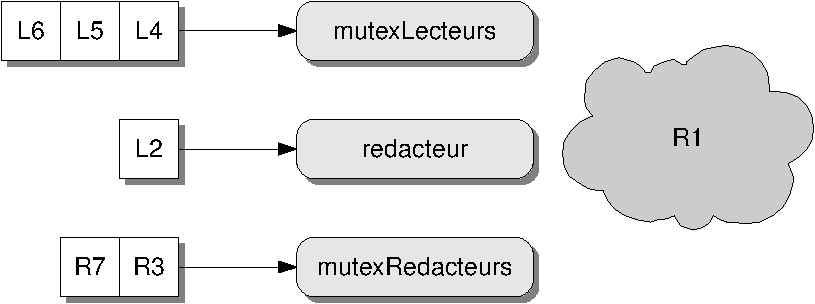
\includegraphics[scale=.7]{lectred1}
    \caption{\label{fig:lectred1}Exemple d'exécution avec priorité aux lecteurs (1)}
  \end{center}
\end{figure}

Lorsque le rédacteur $R1$ libère la ressource, il libère le sémaphore \ccode{redacteur} ce qui permet au premier lecteur d'accéder à la ressource.
Il libère ensuite le sémaphore \ccode{mutexRedacteurs}. Le rédacteur $R3$ se place donc en attente sur le sémaphore \ccode{redacteur}, après le lecteur $L2$.
Le lecteur $L2$ relâche donc le sémaphore \ccode{mutexLecteurs}, ce qui permet à tous les lecteurs en attente d'accéder à la ressource, et le système se retrouve dans l'état illustré par la figure \ref{fig:lectred2}.

\begin{figure}[!ht]
  \begin{center}
    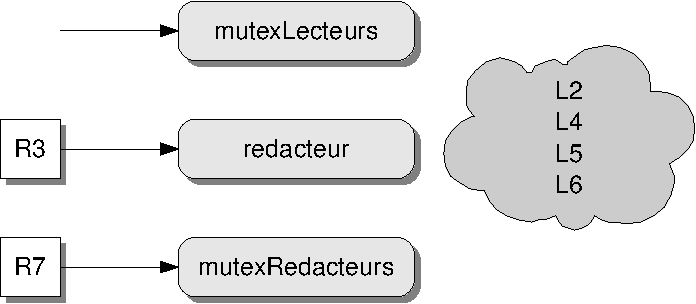
\includegraphics[scale=.7]{lectred2}
    \caption{\label{fig:lectred2}Exemple d'exécution avec priorité aux lecteurs (2)}
  \end{center}
\end{figure}

Lorsque de nouveaux rédacteurs désirent accéder à la ressource, ils sont bloqués par le sémaphore \ccode{mutexRedacteurs}. Les lecteurs désirant effectuer la même action sont par contre autorisés à accéder à la ressource. La figure \ref{fig:lectred3} montre l'état du système après l'arrivée de deux rédacteurs et d'un lecteur. $L9$ se retrouve en accès de ressource, alors que $R8$ et $R10$ sont bloqués.

\begin{figure}[!ht]
  \begin{center}
    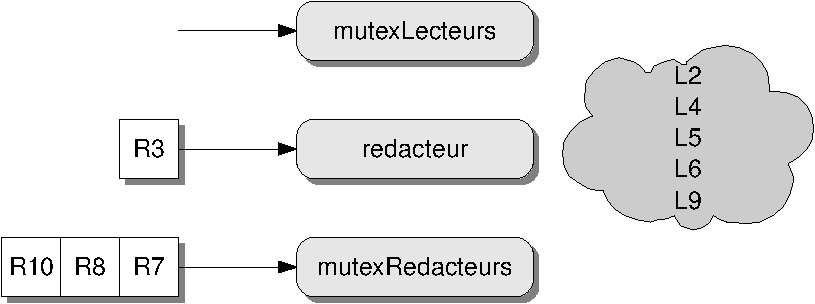
\includegraphics[scale=.7]{lectred3}
    \caption{\label{fig:lectred3}Exemple d'exécution avec priorité aux lecteurs (3)}
  \end{center}
\end{figure}

Lorsque tous les lecteurs ont relâché la ressource, le rédacteur $R3$, qui était bloqué par le sémaphore \ccode{redacteur} peut enfin y avoir accès.
La figure \ref{fig:lectred4} illustre cette situation.
Remarquez que la file d'attente associée à \ccode{redacteur} reste vide car $R3$ bloque toujours les rédacteurs par son sémaphore \ccode{mutexRedacteurs}. Un nouvel lecteur qui se présenterait pourra alors se placer à la tête de cette file et ainsi dépasser tous les rédacteurs présents pour prendre la ressource aussitôt que $R3$ libère \ccode{redacteur}.

\begin{figure}[!ht]
  \begin{center}
    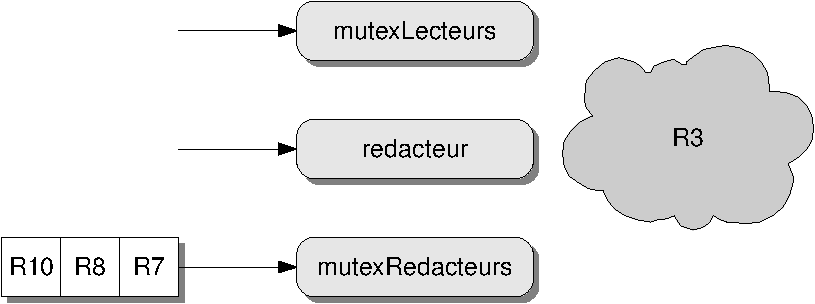
\includegraphics[scale=.7]{lectred4}
    \caption{\label{fig:lectred4}Exemple d'exécution avec priorité aux lecteurs (4)}
  \end{center}
\end{figure}

Nous pouvons noter que cet algorithme permet aux lecteurs de se coaliser pour empêcher l'accès aux rédacteurs. En effet, si un nouveau lecteur accède à la ressource avant que tous les lecteurs ne l'aient relâchée, alors les rédacteurs n'auront jamais accès à la ressource.

Le programme \ref{lectredtest} permet de lancer concurremment des lectures et écritures, et peut être exploité pour l'ensemble des exemples de ce chapitre. Il crée des threads rédacteurs et lecteurs et les laisse tenter d'accéder à une ressource hypothétique. Il est à noter que ce programme ne vérifie pas que l'algorithme est correct. Un exercice en fin de chapitre propose d'y ajouter la vérification.

\begin{algorithm}[h!tp]
\caption{Lecteurs-rédacteurs: Programme de test}\label{lectredtest}
\begin{center}
\begin{tabular}{l}
\lstset{language=C++}
\begin{lstlisting}
#define NUM_THREADS_REDACTEUR   1
#define NUM_THREADS_LECTEUR     3

static RessourceLectRed ressource;

void *tacheRedacteur(void *arg) {
  int tid = (int)arg;
  while (true) {
    debutEcriture(&ressource);
    printf("Tache %d: écriture\n",tid);
    finEcriture(&ressource);
  }
  pthread_exit(NULL);
}

void *tacheLecteur(void *arg) {
  int tid  = (int)arg;
  while (true) {
    debutLecture(&ressource);
    printf("Tache %d: lecture\n",tid);
    finLecture(&ressource);
  }
  pthread_exit(NULL);
}

int main(int argc, char *argv[]) {
  pthread_t threadsRed[NUM_THREADS_REDACTEUR];
  pthread_t threadsLec[NUM_THREADS_LECTEUR];
  int t;
  initialiseRessource(&ressource);
  for (t = 0; t < NUM_THREADS_LECTEUR; t++) {
    printf("Création du lecteur %d\n",t);
    if (pthread_create(&threadsLec[t], NULL, tacheLecteur, (void *)t) == 0)
      exit(-1);
  }
  for (t = 0; t < NUM_THREADS_REDACTEUR; t++) {
    printf("Création du rédacteur %d\n",t);
    if (pthread_create(&threadsRed[t], NULL, tacheRedacteur, (void *)t) == 0)
      exit(-1);
  }
  for (t = 0; t < NUM_THREADS_LECTEUR; t++)
    pthread_join(threadsLec[t],NULL);
  for (t = 0; t < NUM_THREADS_REDACTEUR; t++)
    pthread_join(threadsRed[t],NULL);
  return 0;
}
\end{lstlisting}
\end{tabular}
\end{center}
\end{algorithm}

Nous pouvons également noter que ce programme de test, ainsi la manière dont sont réalisés les différents protocoles présentés dans ce chapitre, peuvent être considérés comme légèrement risqués. En effet, la variable de type \ccode{RessourceLectRed} est déclarée dans le programme principal. En théorie, seules les fonctions de début et de fin de lecture et d'écriture y font référence. Pour que le fonctionnement soit correct, il faudrait garantir que le programme principal n'agisse pas directement sur cette structure, sans quoi le système risquerait de se retrouver dans un état incohérent. Ceci pourrait aisément être réalisé grâce à une meilleure encapsulation, mais la compréhension du chapitre ne nécessitant pas de telles contraintes, l'exercice est laissé au bon vouloir du lecteur.

L'algorithme \ref{lectred:prioritelecteur} peut être légèrement modifié pour donner priorité aux lecteurs uniquement si une lecture est en cours.
Ce nouvel algorithme \ref{lectred:prioritelecteurcourant} permet toujours aux lecteurs de se coaliser, comme précédemment. Si plusieurs rédacteurs veulent accéder à la ressource pendant qu'elle est occupée par des lecteurs, le premier rédacteur accèdera dès que les lecteurs seront tous sortis, mais les rédacteurs en attente auront accès avant les lecteurs futurs. En effet, le prochain lecteur qui se présentera se placera derrière ces rédacteurs et tous ceux qui ont fait une demande avant le lecteur.

\begin{algorithm}[h!tp]
\caption{Lecteurs-rédacteurs: priorité aux lecteurs uniquement si une lecture est en cours}\label{lectred:prioritelecteurcourant}
\begin{center}
\begin{tabular}{l}
\lstset{language=C++}
\begin{lstlisting}
typedef struct {
  sem_t mutexLecteurs;
  sem_t redacteur;
  int nbLecteurs;
} RessourceLectRed;

void initialiseRessource(RessourceLectRed *res) {
  sem_init(&res->mutexLecteurs,0,1);
  sem_init(&res->redacteur,0,1);
  res->nbLecteurs = 0;
}

void debutLecture(RessourceLectRed *res) {
  sem_wait(&res->mutexLecteurs);
  res->nbLecteurs++;
  if (res->nbLecteurs == 1)
    sem_wait(&res->redacteur);
  sem_post(&res->mutexLecteurs);
}

void finLecture(RessourceLectRed *res) {
  sem_wait(&res->mutexLecteurs);
  res->nbLecteurs--;
  if (res->nbLecteurs == 0)
    sem_post(&res->redacteur);
  sem_post(&res->mutexLecteurs);
}

void debutEcriture(RessourceLectRed *res) {
  sem_wait(&res->redacteur);
}

void finEcriture(RessourceLectRed *res) {
  sem_post(&res->redacteur);
}
\end{lstlisting}
\end{tabular}
\end{center}
\end{algorithm}

Il également possible d'implémenter l'algorithme \ref{lectred:prioritelecteur} d'une autre manière. Il s'agit d'un modèle permettant de dériver plusieurs solutions, en fonction des priorités à accorder. Ce modèle de solution se prête également à la résolution de problèmes s'apparentant aux lecteurs-rédacteurs, tels que le passage d'un pont, les giratoires, ou les ressources multiples. Pour ce modèle, nous utilisons les informations contenues dans la structure suivante:

\begin{lstlisting}
typedef struct {
  sem_t mutex;
  sem_t lecteurs;
  sem_t redacteur;
  int nbLecteurs;
  int lectEnAttente;
  int redEnAttente;
  bool unRedacteur;
} RessourceLectRed;
\end{lstlisting}

\begin{itemize}
\item \ccode{mutex} protège l'accès aux variables partagées, tous les threads risquant d'en effectuer des accès concurrents;
\item \ccode{lecteurs} est un sémaphore permettant de bloquer les lecteurs;
\item \ccode{redacteurs} est un sémaphore permettant de bloquer les rédacteurs;
\item \ccode{nbLecteurs} sert à compter le nombre de lecteurs en phase de lecture;
\item \ccode{lectEnAttente} sert à compter le nombre de lecteurs en attente de la ressource;
\item \ccode{redEnAttente} sert à compter le nombre de rédacteurs en attente de la ressource;
\item \ccode{unRedacteur} indique si un rédacteur est en phase d'écriture. Il s'agit d'un booléen, étant donné qu'un seul rédacteur ne peut être en écriture à un instant donné. Cette variable pourrait être un entier dans le cas d'un problème différent de celui du simple lecteurs-rédacteurs.
\end{itemize}

L'algorithme \ref{lectred:prioritelecteurgenerale} présente la solution basée sur ce modèle.

\begin{algorithm}[h!tp]
\caption{Lecteurs-rédacteurs: priorité aux lecteurs, solution générale}\label{lectred:prioritelecteurgenerale}
\begin{center}
\begin{tabular}{l}
\lstset{language=C++}
\begin{lstlisting}
void initialiseRessource(RessourceLectRed *res) {
  sem_init(&res->mutex,0,1);
  sem_init(&res->lecteurs,0,0);
  sem_init(&res->redacteur,0,0);
  res->nbLecteurs = 0;
  res->lectEnAttente = 0;
  res->redEnAttente = 0;
  res->unRedacteur = false;
}

void debutLecture(RessourceLectRed *res) {
  sem_wait(&res->mutex);
  if (res->unRedacteur) {
    res->lectEnAttente++;
    sem_post(&res->mutex);
    sem_wait(&res->lecteurs);
  }
  else {
    res->nbLecteurs++;
    sem_post(&res->mutex);
  }
}

void finLecture(RessourceLectRed *res) {
  sem_wait(&res->mutex);
  res->nbLecteurs--;
  if (res->nbLecteurs == 0 && res->redEnAttente > 0) {
    res->unRedacteur = true;
    res->redEnAttente--;
    sem_post(&res->redacteur);
  }
  sem_post(&res->mutex);
}

void debutEcriture(RessourceLectRed *res) {
  sem_wait(&res->mutex);
  if (res->unRedacteur || res->nbLecteurs + res->lectEnAttente > 0) {
    res->redEnAttente++;
    sem_post(&res->mutex);
    sem_wait(&res->redacteur);
  }
  else {
    res->unRedacteur = true;
    sem_post(&res->mutex);
  }
}

void finEcriture(RessourceLectRed *res) {
  int i;
  sem_wait(&res->mutex);
  res->unRedacteur = false;
  if (res->lectEnAttente > 0) {
    for (i = 0; i < res->lectEnAttente; i++)
      sem_post(&res->lecteurs);
    res->nbLecteurs = res->lectEnAttente;
    res->lectEnAttente = 0;
  }
  else if (res->redEnAttente > 0) {
    res->unRedacteur = true;
    res->redEnAttente--;
    sem_post(&res->redacteur);
  }
  sem_post(&res->mutex);
}
\end{lstlisting}
\end{tabular}
\end{center}
\end{algorithm}


\section{Priorité égale}
Un algorithme basé sur une priorité égale doit résoudre l'accès à la ressource, en respectant les règles suivantes:
\begin{itemize}
\item Un lecteur peut accéder à la ressource uniquement si le nombre de rédacteurs en cours d'écriture vaut 0
\item Un rédacteur peut accéder à la ressource si:
\begin{itemize}
\item le nombre de rédacteurs en cours d'écriture vaut 0
\item ET le nombre de lecteurs en cours de lecture est également 0
\end{itemize}
\end{itemize}

Pour ce faire, nous aurons besoin d'une variable comptant le nombre de lectures en cours: \ccode{nbLecteurs}. Pour garantir l'accès concurrent correct, nous devons également exploiter trois sémaphores.

Les sémaphores nécessaires sont les suivants:
\begin{itemize}
\item \ccode{mutex}, qui est en charge de protéger l'accès à la variable \ccode{nbLecteurs}.
\item \ccode{redacteur}, qui permet au premier lecteur qui accède la ressource de bloquer les futurs rédacteurs. Il permet également au rédacteur accédant la ressource de bloquer les lecteurs pendant l'écriture.
\item \ccode{fifo}, une file d'attente dans laquelle passent tous les lecteurs et rédacteurs.
\end{itemize}

L'algorithme \ref{lectred:prioriteegale} présente une solution avec priorité égale, basée sur ces trois sémaphores.

\begin{algorithm}[h!tp]
\caption{Lecteurs-rédacteurs: priorité égale}\label{lectred:prioriteegale}
\begin{center}
\begin{tabular}{l}
\lstset{language=C++}
\begin{lstlisting}
typedef struct {
  sem_t mutex;
  sem_t fifo;
  sem_t redacteur;
  int nbLecteurs;
} RessourceLectRed;

void initialiseRessource(RessourceLectRed *res) {
  sem_init(&res->mutex,0,1);
  sem_init(&res->fifo,0,1);
  sem_init(&res->redacteur,0,1);
  res->nbLecteurs = 0;
}

void debutLecture(RessourceLectRed *res) {
  sem_wait(&res->fifo);
  sem_wait(&res->mutex);
  res->nbLecteurs++;
  if (res->nbLecteurs == 1)
    sem_wait(&res->redacteur);
  sem_post(&res->mutex);
  sem_post(&res->fifo);
}

void finLecture(RessourceLectRed *res) {
  sem_wait(&res->mutex);
  res->nbLecteurs--;
  if (res->nbLecteurs == 0)
    sem_post(&res->redacteur);
  sem_post(&res->mutex);
}

void debutEcriture(RessourceLectRed *res) {
  sem_wait(&res->fifo);
  sem_wait(&res->redacteur);
}

void finEcriture(RessourceLectRed *res) {
  sem_post(&res->redacteur);
  sem_post(&res->fifo);
}
\end{lstlisting}
\end{tabular}
\end{center}
\end{algorithm}

Le sémaphore \ccode{fifo} est le point central de l'algorithme. Il sert à préserver l'ordre des demandes et il est initialisé à 1, permettant au premier thread arrivé de passer directement. Un seul thread peut donc posséder ce sémaphore à un instant donné, ce qui correspond à un simple verrou. Un seul thread étant en possession du verrou, nous pouvons observer que les rédacteurs acquièrent le verrou dans \ccode{debutEcriture()}, et le relâchent dans \ccode{finEcriture()}. De ce fait, un seul rédacteur ne peut être actif à un instant donné. Du côté des lecteurs, ce même verrou n'est réquisitionné que dans \ccode{debutLecture()}, afin d'autoriser le premier lecteur disponible à accéder la ressource. Le premier à passer va alors bloquer les rédacteurs, grâce au verrou \ccode{redacteur}.

Il est intéressant de noter que les interblocage sont évités grâce
à l'ordre des appels des sémaphores \ccode{fifo} et \ccode{redacteur} qui est effectué pour les lecteurs et les rédacteurs.
Si tel n'avait pas été le cas, le système aurait risqué un interblocage.

\section{Priorité aux rédacteurs}
Un algorithme basé sur une priorité aux rédacteurs doit résoudre l'accès à la ressource, en respectant les règles suivantes:
\begin{itemize}
\item Un lecteur peut accéder à la ressource si:
\begin{itemize}
\item le nombre de rédacteurs en cours d'écriture vaut 0
\item ET le nombre de rédacteurs en attente d'écriture vaut également 0
\end{itemize}
\item Un rédacteur peut accéder à la ressource si:
\begin{itemize}
\item le nombre de rédacteurs en cours d'écriture vaut 0
\item ET le nombre de lecteurs en cours de lecture vaut également 0
\end{itemize}
\end{itemize}

Dans ce cas, à l'instar des lecteurs dans le cas d'une priorité les avantageant, les rédacteurs pourront se coaliser pour empêcher les lecteurs d'accéder à la ressource.

Pour cet algorithme, nous aurons besoin d'une variable comptant le nombre de lectures en cours, \ccode{nbLecteurs}, ainsi qu'une comptant le nombre de rédacteurs en attente d'écriture ou en cours d'écriture. Pour garantir l'accès concurrent correct, nous devons également exploiter cinq sémaphores.

Les sémaphores nécessaires sont donc les suivants:
\begin{itemize}
\item \ccode{mutexLecteurs}, qui permet de bloquer les lecteurs pendant que des écritures sont en cours.
\item \ccode{mutexRedacteurs}, qui permet de bloquer les rédacteurs pendant que des écritures ou des lectures sont en cours.
\item \ccode{redacteur}, qui permet au premier lecteur qui accède la ressource de bloquer les potentiels rédacteurs.
\item \ccode{lecteur}, qui permet au premier rédacteur arrivé de bloquer les potentiels futurs lecteurs.
\item \ccode{mutex}, qui est en charge de protéger l'accès à la variable \ccode{nbLecteurs}.
\end{itemize}

L'algorithme \ref{lectred:prioriteredacteurs} présente une solution avec priorité aux rédacteurs, basée sur ces cinq sémaphores.


\begin{algorithm}[h!tp]
\caption{Lecteurs-rédacteurs: priorité aux rédacteurs}\label{lectred:prioriteredacteurs}
\begin{center}
\begin{tabular}{l}
\lstset{language=C++}
\begin{lstlisting}
typedef struct {
  sem_t mutexLecteurs;
  sem_t mutexRedacteurs;
  sem_t lecteur;
  sem_t redacteur;
  sem_t mutex;
  int nbLecteurs;
  int nbRedacteurs;
} RessourceLectRed;

void initialiseRessource(RessourceLectRed *res) {
  sem_init(&res->mutexLecteurs,0,1);
  sem_init(&res->mutexRedacteurs,0,1);
  sem_init(&res->redacteur,0,1);
  sem_init(&res->lecteur,0,1);
  sem_init(&res->mutex,0,1);
  res->nbLecteurs = 0;
  res->nbRedacteurs = 0;
}

void debutLecture(RessourceLectRed *res) {
  sem_wait(&res->mutexLecteurs);
  sem_wait(&res->lecteur);
  sem_wait(&res->mutex);
  res->nbLecteurs++;
  if (res->nbLecteurs == 1)
    sem_wait(&res->redacteur);
  sem_post(&res->mutex);
  sem_post(&res->lecteur);
  sem_post(&res->mutexLecteurs);
}

void finLecture(RessourceLectRed *res) {
  sem_wait(&res->mutex);
  res->nbLecteurs--;
  if (res->nbLecteurs == 0)
    sem_post(&res->redacteur);
  sem_post(&res->mutex);
}

void debutEcriture(RessourceLectRed *res) {
  sem_wait(&res->mutexRedacteurs);
  res->nbRedacteurs++;
  if (res->nbRedacteurs == 1)
    sem_wait(&res->lecteur);
  sem_post(&res->mutexRedacteurs);
  sem_wait(&res->redacteur);
}

void finEcriture(RessourceLectRed *res) {
  sem_post(&res->redacteur);
  sem_wait(&res->mutexRedacteurs);
  res->nbRedacteurs--;
  if (res->nbRedacteurs == 0)
    sem_post(&res->lecteur);
  sem_post(&res->mutexRedacteurs);
}
\end{lstlisting}
\end{tabular}
\end{center}
\end{algorithm}

Nous pouvons noter une certaine symétrie entre les lecteurs et les rédacteurs, chacuns étant capables de bloquer les autres. Le premier lecteur à accéder à la ressource bloque les rédacteurs, grâce au sémaphore \ccode{redacteur}. En fin de lecture, le dernier lecteur à relâcher la ressource va alors débloquer les rédacteurs. De manière symétrique, le premier rédacteur à accéder à la ressource va bloquer l'ensemble des lecteurs grâce au sémaphore \ccode{lecteur}, et le dernier rédacteur à relâcher la ressource va débloquer les lecteurs.

\section{Conclusion}

Le problème des lecteurs-rédacteurs peut être résolu de différentes manières, tel que démontré par les deux algorithmes pour la priorité aux lecteurs. Ce paradigme peut également servir à modéliser différents types de systèmes tels que l'accès à un pont à voie unique par des voitures venant des deux sens, par exemple. De tels problèmes seront abordés en exercices.


\section{Exercices}

\startexercice

Dans l'algorithme \ref{lectred:prioritelecteur}, pourrions-nous remplacer les sémaphores par des verrous? Montrer comment.

\startexercice

Reprendre l'algorithme général avec priorité aux lecteurs (algorithme \ref{lectred:prioritelecteurgenerale}), et l'adapter pour proposer une nouvelle solution qui donne priorité aux rédacteurs.

\startexercice

Mettre au point un programme capable de tester un des algorithmes présentés dans ce chapitre.

\startexercice

Une application est composée de threads de deux classes, A et B. Une ressource est partagée entre tous les threads, selon les contraintes suivantes:
\begin{enumerate}
\item Les threads de classe A peuvent accéder concurremment  à la ressource.
\item Les threads de classe B peuvent accéder concurremment à la ressource.
\item Les threads de différente classe ne peuvent accéder à la ressource au même instant. Autrement dit, les threads de différente classe s'excluent mutuellement.
\end{enumerate}

Proposer un algorithme permettant de gérer l'accès à la ressource, en s'inspirant des solutions du chapitre. Considérer une solution où la coalition est possible entre threads d'une même classe.

%\subsection*{Exercice 6}
%En reprenant l'algorithme précédent, proposer une solution où la coalition n'est pas tolérée. La séquence d'accès doit donc y être respectée.
%CEZ: Je ne comprend pas: c'est l'algo égalitaire!

\startexercice

Proposer un scénario semblable aux figures \ref{fig:lectred1} à \ref{fig:lectred4}, illustrant le fonctionnement de l'algorithme
\ref{lectred:prioritelecteurcourant}, où les lecteurs sont prioritaires que si une lecture est en cours.

\chapter{Moniteurs}
\startchapter
\lettrine[lines=4]{L}es mécanismes de coopération et de synchronisation basés sur les verrous et les sémaphores constituent des constructions non structurées. Ces mécanismes sont donc difficiles à mettre en oeuvre et il est délicat de prouver leur fiabilité ou le respect des contraintes d'un cahier des charges. Afin de pallier à ces points faibles, de nouvelles constructions et de nouvelles abstractions ont successivement été proposées. Parmi les propositions, on relève les moniteurs permettant de mettre en oeuvre une synchronisation orientée sur les données. Les moniteurs ont été implémentés dans divers langages de programmation concurrente: Pascal Concurrent, Modula, Portal et même plus récemment $\mu$C++ ainsi que Java.
\section{Définition}
Un {\em moniteur} comprend un ensemble de variables et un ensemble de procédures qui manipulent ces variables. Certaines procédures sont accessibles depuis l'extérieur et sont les {\em points d'entrée} du moniteur. Les tâches qui font appel à un moniteur pour se synchroniser n'ont pas un accès direct aux variables contenues dans le moniteur. Elles ne peuvent les atteindre que par les points d'entrée fournis par le moniteur. Les procédures contiennent des opérations qui permettent de bloquer et de réveiller les tâches conformément aux spécifications du problème. Les conditions de blocage et de réveil sont exprimées en fonction des variables du moniteur. Le mécanisme d'exécution du moniteur garantit qu'une seule tâche est active dans le moniteur, en train d'exécuter une de ses procédures. Un moniteur contient aussi une partie d'initialisation qui n'est exécutée qu'une fois lors de la création du moniteur (voir figure~\ref{moniteur:struct}). Un moniteur est donc tout simplement un type de donnée abstrait qui possède des mécanismes de synchronisation et dont l'accès se réalise en exclusion mutuelle.
\begin{figure}[!ht]

\begin{center}
\begin{tabular}{l}
{\bf monitor} <{\em nom}> \\
\hspace{0.3cm}<{\em déclarations des variables rémanentes locales}>; \\
\hspace{0.3cm}<{\em déclarations des variables conditions}>;  \\
\hspace{0.3cm}{\bf procedure} {\em OpérationLocale}({\em liste de paramètres)}  \\
\hspace{0.6cm}<{\em déclarations des variables locales}>; \\
\hspace{0.6cm}{\bf begin} <{\em code pour implémenter l'opération}>; \\
\hspace{0.6cm}{\bf end}; \\
\hspace{0.3cm}{\bf entry procedure} {\em OpérationVisible}({\em liste de paramètres}) \\
\hspace{0.6cm}<{\em déclarations des variables locales}>; \\
\hspace{0.6cm}{\bf begin} <{\em code pour implémenter l'opération}>; \\
\hspace{0.6cm}{\bf end}; \\
\hspace{0.3cm}{\bf begin} <{\em code pour initialiser les variables rémanentes}>; \\
\hspace{0.3cm}{\bf end};
\end{tabular}
\caption{\label{moniteur:struct}Structure d'un moniteur}
\end{center}
\end{figure}

La synchronisation des tâches s'exprime au moyen de {\em variables conditions} (VC). Une VC est déclarée comme une variable ordinaire mais elle ne peut être utilisée que par 2 primitives: les primitives {\em attente} et {\em signale}. Soit la VC $cond$ déclarée par
\begin{center}
{\bf condition} $cond$;
\end{center}
les opérations $cond.attente$ et $cond.signale$ ont les effets suivants. La primitive $cond.attente$ bloque inconditionnellement la tâche appelante, lui fait relâcher l'exclusion mutuelle sur le moniteur et la place dans une file associée à $cond$. Le résultat de l'exécution de la primitive $cond.signale$ dépend de l'état de la file associée à $cond$. Si la file est vide, la tâche appelante poursuit son exécution et l'opération n'a aucun effet.  Aucun état n'est préservé par la VC, à la différence de l'opération $V$ qui affecte l'état du sémaphore. Par contre si la file associée à $cond$ n'est pas vide, l'une des tâches bloquées est réactivée et reprend immédiatement son exécution à l'instruction qui suit la primitive $cond.attente$. La tâche appelante est suspendue et reprendra son exécution lorsque la tâche qu'elle a réveillée exécute une primitive $attente$ ou quitte le moniteur.

Prenons quelques exemples pour illustrer ces idées. L'algorithme~\ref{moniteur:exempleVerrou} montre une implémentation d'un verrou. La variable \ccode{verrou} indique l'état du verrou. La première exécution de \ccode{Verrouille} met \ccode{verrou} à vrai. Les appels de \ccode{Verrouille} suivants bloqueront les tâches appelantes.  Remarquons que la procédure \ccode{Deverrouille} essaie toujours de réveiller une tâche en attente après avoir modifié \ccode{verrou}. Si une telle tâche existe, cette tâche remet immédiatement \ccode{verrou} à vrai, sinon \ccode{verrou} reste inchangée.

\begin{algorithm}[!htb]
\caption{Verrou par moniteur}\label{moniteur:exempleVerrou}
\begin{center}
\begin{tabular}{l}
{\bf monitor} VerrouMoniteur \\
\hspace{0.3cm}{\bf var} verrou: boolean; \\
\hspace{0.3cm}{\bf var} acces: {\bf condition}; \\

\hspace{0.3cm}{\bf entry procedure} Verrouille \\
\hspace{0.6cm}{\bf begin} \\
\hspace{1cm} {\bf if} verrou {\bf then} acces.attente; \\
\hspace{1cm} verrou := {\em true}; \\
\hspace{0.6cm}{\bf end} Verrouille; \\

\hspace{0.3cm}{\bf entry procedure} Deverrouille \\
\hspace{0.6cm}{\bf begin} \\
\hspace{1cm}verrou := {\em false}; \\
\hspace{1cm}acces.signale; \\
\hspace{0.6cm}{\bf end} Deverrouille; \\

\hspace{0.3cm}{\bf begin} verrou := {\em false}; \\
\hspace{0.3cm}{\bf end} VerrouMoniteur;
\end{tabular}
\end{center}
\end{algorithm}
\par
Le problème des producteurs et des consommateurs, illustré sur l'algorithme~\ref{moniteur:ProdCons}, est rendu évident. Signalons seulement le fait que lors de la création du moniteur, la partie d'initialisation doit se faire avant tout appel à l'une des procédures accessibles du moniteur.
\begin{algorithm}[!ht]
\caption{Problème des producteurs et des consommateurs par moniteur}\label{moniteur:ProdCons}
\begin{center}
\begin{tabular}{l}
{\bf monitor} Tampons \\
\hspace{0.3cm}{\bf var} place: array [0..N-1] {\bf of} ARTICLE; \\
\hspace{0.3cm}{\bf var} tete, queue, taille: integer; \\
\hspace{0.3cm}{\bf var} pasPlein, pasVide: {\bf condition}; \\

\hspace{0.3cm}{\bf entry procedure} deposer(a: ARTICLE) \\
\hspace{0.6cm}{\bf begin} \\
\hspace{1cm}{\bf if} taille = N {\bf then} pasPlein.attente; \\
\hspace{1cm}taille := taille + 1; \\
\hspace{1cm}place[tete] := a; \\
\hspace{1cm}tete := (tete + 1) {\bf mod} N; \\
\hspace{1cm}pasVide.signale; \\
\hspace{0.6cm}{\bf end} deposer; \\

\hspace{0.3cm}{\bf entry procedure} retirer({\bf var} a: ARTICLE) \\
\hspace{0.6cm}{\bf begin} \\
\hspace{1cm}{\bf if} taille = 0 {\bf then} pasVide.attente; \\
\hspace{1cm}a := place[queue]; \\
\hspace{1cm}taille := taille - 1; \\
\hspace{1cm}queue := (queue + 1) {\bf mod} N; \\
\hspace{1cm}pasPlein.signale; \\
\hspace{0.6cm}{\bf end} retirer; \\

\hspace{0.3cm}{\bf begin} taille := 0; queue := 0; tete := 0; \\
\hspace{0.3cm}{\bf end} Tampons;
\end{tabular}
\end{center}
\end{algorithm}
\par
Attardons-nous à présent sur quelques extensions et sur quelques variantes du modèle des moniteurs que nous avons introduit. Lorsqu'une tâche $Q$ se fait réveiller par la primitive {\em signale}, $Q$ reprend immédiatement son exécution. Cette approche est la plus répandue car la condition sur laquelle $Q$ était en attente est toujours vérifiée lorsque $Q$ reprend son exécution. Certains langages abordent la question différemment.  Par exemple en Mesa, l'ancêtre de Java, la primitive {\em notify} exécutée par la tâche $P$ sur une VC a pour effet de réveiller une tâche, mais cette dernière ne reprendra son exécution seulement après que $P$ libère le moniteur. Ainsi en Mesa, la mise en suspension s'écrit par  \\
\hspace*{1cm}{\bf while} B {\bf do}  \\
\hspace*{1.3cm}VC.attente;  \\
\hspace*{1cm}{\bf end};  \\
au lieu de  \\
\hspace*{1cm}{\bf if} B {\bf then}  VC.attente; \\
Cette approche a deux extensions intéressantes. D'abord un chien de garde peut être associé à chaque VC. Si une tâche est suspendue plus longtemps qu'elle ne devrait, le système peut émettre automatiquement un {\em notify} et la tâche ainsi réveillée peut alors effectuer les actions appropriées. Enfin la primitive {\em broadcast} généralise la primitive {\em notify} et a pour effet de réveiller toutes les tâches qui sont suspendues sur la VC. Le choix de la tâche qui reprend contrôle du moniteur, une fois que celui-ci devient libre, est laissé au soin du répartiteur. La gestion des tâches est ainsi simplifiée.

\section{Moniteurs en $pthreads$}
Les moniteurs $pthreads$ sont réalisés en conjuguant verrous et variables conditions.
\subsection*{Rappel}
Création d'un verrou \\
\hspace*{1cm}\ccode{int pthread_mutex_init(pthread_mutex_t *m,} \\
\hspace*{5cm}\ccode{ const pthread_mutex_attr *attr)} \\
ou \\
\hspace*{1cm}\ccode{pthread_mutex_t m = PTHREAD_MUTEX_INITIALIZER;} \\
Destruction d'un verrou \\
\hspace*{1cm}\ccode{int pthread_mutex_destroy(pthread_mutex_t *mutex)} \\
Verrouillage, avec blocage en attente si déjà verrouillé. Renvoie 0 si tout se passe bien. \\
\hspace*{1cm}\ccode{int pthread_mutex_lock(pthread_mutex_t *mutex)} \\
Déverrouillage. Seule la tâche qui a verrouillé le verrou a le droit de le déverrouiller (en cas de tentative de déverrouiller un verrou verrouillé par une autre tâche, le comportement est indéfini). \\
\hspace*{1cm}\ccode{int pthread_mutex_unlock(pthread_mutex_t *mutex)} \\
Si une ou plusieurs tâches sont bloquées, en attente du verrou, une d'entre elles obtient le verrou et est débloquée. Le choix de cette tâche dépend des priorités et des politiques d'ordonnancement. Si les attributs (pour la création des tâches et des verrous) ne sont pas utilisés, l'ordre de déblocage est indéterminé (pas nécessairement FIFO).

\subsection*{Variables conditions}
\begin{enumerate}
\item Création d'une variable condition \\
\hspace*{1cm}\ccode{int pthread_cond_init(pthread_cond_t *c,} \\
\hspace*{5cm}\ccode{ const pthread_cond_attr *attr)} \\
ou \\
\hspace*{1cm}\ccode{pthread_cond_t c = PTHREAD_COND_INITIALIZER;} \\
Crée la variable condition \ccode{c} (on ignorera l'attribut).
\item Destruction d'une variable condition \\
\hspace*{1cm}\ccode{int pthread_cond_destroy(pthread_cond_t *c)} \\
Détruit la variable condition \ccode{c}.
\item Mise en attente inconditionnelle \\
\hspace*{1cm}\ccode{int pthread_cond_wait(pthread_cond_t *cond,}\\
\hspace*{5cm}\ccode{ pthread_mutex_t *mutex)} \\
La tâche appelante doit posséder le verrou \ccode{mutex}. La tâche est alors bloquée sur la variable condition \ccode{cond} après avoir libéré le verrou, et la tâche reste bloquée jusqu'à ce que la variable condition soit signalée et que la tâche réussisse à réacquérir le verrou.
\item Réveil d'une tâche \\
\hspace*{1cm}\ccode{int pthread_cond_signal(pthread_cond_t *cond)} \\
Signale la variable condition : une tâche bloquée sur la variable condition \ccode{cond} est réveillée. Cette tâche tente alors de réacquérir le verrou correspondant à son appel de \ccode{pthread_cond_wait}. Elle sera effectivement débloquée quand elle réussira à réacquérir ce verrou. Il n'y a aucun ordre garanti pour le choix de la tâche réveillée. Aussi, l'opération \ccode{pthread_cond_signal} n'a aucun effet s'il n'y a aucune tâche bloquée sur la variable condition (pas de mémorisation). \\
\hspace*{1cm}\ccode{int pthread_cond_broadcast(pthread_cond_t *cond)} \\
Toutes les tâches en attente sont réveillées et tentent d'obtenir le verrou correspondant à leur appel de \ccode{pthread_cond_wait}.
\end{enumerate}

\subsection*{Remarques}
Contrairement à la définition des moniteurs que nous avons vu précédemment, la tâche signalée n'a pas priorité sur le signaleur : le signaleur ne perd pas l'accès au moniteur s'il le possédait, et le signalé reste bloqué tant qu'il n'obtient pas le verrou. C'est pourquoi il est nécessaire d'utiliser une boucle d'attente réévaluant la condition d'exécution. En effet, cette condition peut être invalidée entre le moment où la tâche est signalée et le moment où elle obtient effectivement le verrou, par exemple si une autre tâche obtient le verrou et pénètre dans le moniteur avant la tâche signalée.

Enfin, pour des raisons d'efficacité, il est courant de faire l'appel à \ccode{pthread_cond_signal} hors de la zone d'exclusion mutuelle du moniteur, de sorte que la tâche signalée puisse acquérir plus facilement le verrou. Attention cependant à garantir l'atomicité des opérations du moniteur!

L'algorithme \ref{moniteurs:pthreadProdCons} propose une solution au problème des producteurs et des consommateurs grâce aux primitives proposées par la bibliothèque {\em pthread}.

\begin{algorithm}[!ht]
\caption{Exemple d'un moniteur $pthread$: problème des producteurs et des consommateurs à un tampon}\label{moniteurs:pthreadProdCons}
\begin{center}
\begin{tabular}{l}
\lstset{language=C++}
\begin{lstlisting}
#include <pthread.h>
#include <string.h>
#include <stdlib.h>
static pthread_cond_t estLibre, estPlein;
static pthread_mutex_t protege;
static char *tampon = NULL;

/* Initialise le producteur/consommateur. */
void InitialiseTampon(void)
{
  pthread_mutex_init(&protege,NULL);
  pthread_cond_init(&estLibre,NULL);
  pthread_cond_init(&estPlein,NULL);
} /* fin de InitialiseTampon */

/* Depose le message msg (qui est dupliqué) et bloque tant que le
** tampon est plein. */
void Deposer(char *msg) {
  pthread_mutex_lock(&protege);
  while (tampon != NULL)
     pthread_cond_wait(&estLibre,&protege);
  if ((tampon = (char *)malloc(strlen(msg) + 1)) != NULL) {
     strcpy(tampon,msg);
     pthread_cond_signal(&estPlein);
  }
  pthread_mutex_unlock(&protege);
} /* fin de Deposer */

/* Renvoie le message du tampon et bloque tant que le tampon est vide.
** La libération de la mémoire contenant le message est à la charge de
** l'appelant. */
char *Prelever(void) {
  char *resultat;
  pthread_mutex_lock(&protege);
  while (buffer == NULL)
     pthread_cond_wait(&estPlein,&protege);
  resultat = tampon;
  tampon = NULL;
  pthread_mutex_unlock(&protege);
  pthread_cond_signal(&estLibre);
  return resultat;
} /* fin de Prelever */

void DetruitTampon(void) {
  pthread_mutex_destroy(&protege);
  pthread_cond_destroy(&estLibre);
  pthread_cond_destroy(&estPlein);
  if (tampon != NULL) {
     free(tampon);
     tampon = NULL;
  }
} /* fin de DetruitTampon */
\end{lstlisting}
\end{tabular}
\end{center}
\end{algorithm}

\section{Implémentation de moniteurs à partir de sémaphores}

L'implémentation de moniteurs à l'aide de sémaphores se réalise de la manière suivante.  Une structure de données est associée à chaque variable de type moniteur.
La procédure à appliquer comporte 5 étapes.
\begin{enumerate}
\item Pour chaque variable (instance) $mon$ de type moniteur, créer un enregistrement : \\
\hspace*{0.3cm}\ccode{typedef struct \{ } \\
\hspace*{0.7cm}\ccode{      sem_t mutex; } \\
\hspace*{0.7cm}\ccode{      sem_t signale;       // file bloquante des signaleurs } \\
\hspace*{0.7cm}\ccode{      unsigned nbSignale; // tâches en attente dans signale } \\
\hspace*{0.3cm}\ccode{ \} T_Moniteur; } \\
\hspace*{0.3cm}\ccode{T_Moniteur mon; } \\
Le sémaphore \ccode{mutex} assure l'exclusion mutuelle du moniteur et le sémaphore \ccode{signale} bloque, si nécessaire, les processus qui exécutent la primitive $signale$ sur n'importe quelle VC déclarée dans le moniteur.  La variable \ccode{nbSignale} comptabilise le nombre de tâches suspendues sur le sémaphore \ccode{signale}.

\item Chaque procédure constituant un point d'entrée du moniteur est encadré par : \\
\hspace*{0.3cm}\ccode{sem_wait(&mon.mutex); } \\
\hspace*{0.3cm}< {\em code de la procédure}>  \\
\hspace*{0.3cm}\ccode{if (mon.nbSignale > 0) sem_post(&mon.signale); } \\
\hspace*{0.3cm}\ccode{else sem_post(&mon.mutex); } \\
L'exclusion mutuelle est assurée par le sémaphore {mutex}, et lors du relâchement du moniteur, la priorité est donnée à la tâche ayant émis un $signale$.

\item Pour chaque variable condition \ccode{cond} du moniteur, créer un enregistrement: \\
\hspace*{0.3cm}\ccode{typedef struct \{ } \\
\hspace*{0.7cm}\ccode{      sem_t attente; } \\
\hspace*{0.7cm}\ccode{      unsigned nbAttente; // tâches en attente } \\
\hspace*{0.3cm}\ccode{ \} T_Condition; } \\
\hspace*{0.3cm}\ccode{T_Condition cond; }

\item Dans toutes les procédures du moniteur, substituer \ccode{cond.attente} par :
\hspace*{0.3cm}\ccode{cond.nbAttente += 1; } \\
\hspace*{0.3cm}\ccode{if (mon.nbSignale > 0) sem_post(&mon.signale); } \\
\hspace*{0.3cm}\ccode{else sem_post(&mon.mutex); } \\
\hspace*{0.3cm}\ccode{sem_wait(&cond.attente); } \\
\hspace*{0.3cm}\ccode{cond.nbAttente -= 1; }

\item Dans toutes les procédures du moniteur, substituer \ccode{cond.signale} par :\\
\hspace*{0.3cm}\ccode{if (cond.nbAttente > 0) \{ } \\
\hspace*{0.7cm}\ccode{mon.nbSignale += 1; } \\
\hspace*{0.7cm}\ccode{sem_post(&cond.attente); } \\
\hspace*{0.7cm}\ccode{sem_wait(mon.signale); } \\
\hspace*{0.7cm}\ccode{mon.nbSignale -= 1;} \\
\hspace*{0.3cm}\ccode{ \} }
\end{enumerate}

Pour illustrer l'utilité des substitutions ci-dessus, prenons l'algorithme~\ref{moniteur:ProdCons} montrant la gestion des tampons entre producteurs et consommateurs. Après application directe des substituons, nous obtenons l'algorithme~\ref{moniteur:ProdCons2}.
\begin{algorithm}[!ht]
\caption{Problème des producteurs et des consommateurs à un tampon (sans optimisation)}\label{moniteur:ProdCons2}
\begin{center}
\begin{tabular}{l}
\lstset{language=C++}
\begin{lstlisting}
static T_Moniteur Tampons;
static ARTICLE place[0..N-1];
static int tete, queue, taille;
static T_Condition pasPlein, pasVide;

void deposer(ARTICLE a) {
  sem_wait(&Tampons.mutex);
  if (taille == N) {
     pasPlein.nbAttente += 1;
     if (Tampons.nbSignale > 0)
        sem_post(&Tampons.signale);
     else sem_post(&Tampons.mutex);
     sem_wait(&pasPlein.attente);
     pasPlein.nbAttente -= 1;
  }
  taille += 1;
  place[tete] = a;
  tete = (tete + 1) % N;
  if (pasVide.nbAttente > 0) {
     Tampons.nbSignale += 1;
     sem_post(&pasVide.attente);
     sem_wait(Tampons.signale);
     Tampons.nbSignale -= 1;
  }
  if (Tampons.nbSignale > 0)
     sem_post(&Tampons.signale);
  else
     sem_post(&Tampons.mutex);
} /* fin de deposer */

void retirer(ARTICLE *a) {
  sem_wait(&Tampons.mutex);
  if (taille == 0) {
     pasVide.nbAttente += 1;
     if (Tampons.nbSignale > 0)
        sem_post(&Tampons.signale);
     else sem_post(&Tampons.mutex);
     sem_wait(&pasVide.attente);
     pasVide.nbAttente -= 1;
  }
  a = place[queue];
  taille -= 1;
  queue = (queue + 1) % N;
  if (pasPlein.nbAttente > 0) {
     Tampons.nbSignale += 1;
     sem_post(&pasPlein.attente);
     sem_wait(Tampons.signale);
     Tampons.nbSignale -= 1;
  }
  if (Tampons.nbSignale > 0)
     sem_post(&Tampons.signale);
  else
     sem_post(&Tampons.mutex);
} /* fin de retirer */
\end{lstlisting}
\end{tabular}
\end{center}
\end{algorithm}

Malgré que la substitution obtenue donne une solution correcte, celle-ci peut être optimisée. Lorsqu'un producteur dépose un article et réveille un consommateur (\ccode{pasVide.signale}), ce producteur se met en attente dans la file des signaleurs, puis quand le contrôle lui revient, il sort du moniteur. Pour ce producteur, il aurait été préférable de réveiller le consommateur et de sortir immédiatement. La procédure \ccode{deposer} devient alors %\vspace*{-0.6cm}
\begin{center}
\begin{tabular}{l}
\lstset{language=C++}
\begin{lstlisting}
void deposer(ARTICLE a) {
  sem_wait(&Tampons.mutex);
  if (taille == N) {
     pasPlein.nbAttente += 1;
     if (Tampons.nbSignale > 0)
        sem_post(&Tampons.signale);
     else sem_post(&Tampons.mutex);
     sem_wait(&pasPlein.attente);
     pasPlein.nbAttente -= 1;
  }
  taille += 1;
  place[tete] = a;
  tete = (tete + 1) % N;
  if (pasVide.nbAttente > 0)
     sem_post(&pasVide.attente);
  else if (Tampons.nbSignale > 0)
     sem_post(&Tampons.signale);
  else
     sem_post(&Tampons.mutex);
} /* fin de deposer */
\end{lstlisting}
\end{tabular}
\end{center}
Finalement, on constate qu'après cette transformation la file \ccode{signale} est toujours vide. Nous pouvons éliminer tout ce qui est en relation avec le sémaphore \ccode{signale}. La version finale est donnée sur l'algorithme~\ref{moniteur:ProdCons3},  où nous avons appliqué les mêmes transformations à la procédure \ccode{retirer}.

\begin{algorithm}[!ht]
\caption{Problème des producteurs et des consommateurs à un tampon (version finale)}\label{moniteur:ProdCons3}
\begin{center}
\begin{tabular}{l}
\lstset{language=C++}
\begin{lstlisting}
static T_Moniteur Tampons;
static ARTICLE place[0..N-1];
static int tete, queue, taille;
static T_Condition pasPlein, pasVide;

void deposer(ARTICLE a) {
  sem_wait(&Tampons.mutex);
  if (taille == N) {
     pasPlein.nbAttente += 1;
     sem_post(&Tampons.mutex);
     sem_wait(&pasPlein.attente);
     pasPlein.nbAttente -= 1;
  }
  taille += 1;
  place[tete] = a;
  tete = (tete + 1) % N;
  if (pasVide.nbAttente > 0)
     sem_post(&pasVide.attente);
  else
     sem_post(&Tampons.mutex);
} /* fin de deposer */

void retirer(ARTICLE *a) {
  sem_wait(&Tampons.mutex);
  if (taille == 0) {
     pasVide.nbAttente += 1;
     sem_post(&Tampons.mutex);
     sem_wait(&pasVide.attente);
     pasVide.nbAttente -= 1;
  }
  a = place[queue];
  taille -= 1;
  queue = (queue + 1) % N;
  if (pasPlein.nbAttente > 0)
     sem_post(&pasPlein.attente);
  else
     sem_post(&Tampons.mutex);
} /* fin de retirer */
\end{lstlisting}
\end{tabular}
\end{center}
\end{algorithm}

\section{Remarques finales}
Grâce à leur construction haut niveau, les moniteurs procurent les avantages suivants:
\begin{itemize}
\item[-] une protection associée au moniteur (exclusion mutuelle);
\item[-] une souplesse d'utilisation des primitives $attente$ et $signale$;
\item[-] une efficacité de ces mécanismes.
\end{itemize}
Les moniteurs ont aussi quelques inconvénients:
\begin{itemize}
\item[-] un risque de manque de lisibilité qui est partiellement dû à des variations sémantiques des implémentations dans les divers langages qui les supportent. Dans le cas de $pthread$, il n'y a aucune garantie que les variables partagées sont effectivement accédées uniquement depuis les points d'entrée du moniteur qui devrait les protéger;
\item[-] les variables condition sont de bas niveau;
\item[-] l'impossibilité d'imposer un ordre total ou partiel dans l'exécution des procédures ou fonctions exportées.
\end{itemize}


\section{Exercices}

\startexercice

Proposer une solution au problème des lecteurs/rédacteurs avec priorité aux lecteurs, en faisant appel au concept de moniteur. Donnez une solution avec verrou et variable condition, puis transformez-là en une solution à base de sémaphores.

\startexercice

Considérons le problème des producteurs/consommateurs, où les consommateurs consomment obligatoirement deux données avant de poursuivre leur exécution.

Proposer une solution basée sur les moniteurs.

\startexercice

Considérons le problème des producteurs/consommateurs, où les consommateurs consomment obligatoirement deux données avant de poursuivre leur exécution. Attention, deux données déposées successivement par les producteurs doivent être consommées par le même consommateur avant que le consommateur suivant puisse commencer ses consommations.

Proposer une solution basée sur les moniteurs.


\appendix

\newcommand{\function}[1]{\section{#1}}

\chapter{Bibliothèque Pthread}
\startchapter

Le langage C n'offre pas de mécanisme natif de gestion des threads. Toutefois, il existe des bibliothèques spécifiques qui accomplissent ce rôle. Dans ce qui suit, nous nous tardons sur l'une d'elles, la bibliothèque \emph{Pthread}.

En POSIX (ISO/IEC 9945-1$:$1996), les tâches et les outils de synchronisation font partie de la bibliothèque Pthread.
La bibliothèque Pthread est portable; elle existe sur Linux ainsi que sur Windows. Pour Windows, il faudra cependant l'installer car elle ne l'est pas par défaut. Pour cela, il faudra la télécharger depuis le site

\hspace{1cm}\url{http://sourceware.org/pthreads-win32/}.

Les définitions des types, des fonctions et des constantes se trouvent dans le fichier en-tête pthread.h. A l'édition des liens, il faut aussi préciser cette bibliothèque, par exemple par

\hspace{1cm}\ccode{gcc monapplication.c -lpthread}

Sur certaines plateformes, il faut aussi spécifier au compilateur la constante symbolique \ccode{_REENTRANT}:

\hspace{1cm}\ccode{gcc -D_REENTRANT monapplication.c -lpthread}

Pour pouvoir utiliser un thread, il est nécessaire de déclarer une variable de type \ccode{pthread_t}. Ce type est en fait un entier qui correspond à l'identificateur du thread utilisé. Sur Linux il s'agit en général du type \ccode{unsigned long}. Par exemple:

\hspace{1cm}\ccode{pthread_t thread;}

En plus de la manipulation de threads, POSIX met aussi à disposition un mécanisme de verrous pour réaliser des sections critiques. Si un thread possède le verrou, seulement celui-ci peut accéder à la section critique, et lorsque le thread quitte cette section de code, il libère le verrou et un autre thread peut le prendre à son tour. Pour créer un verrou, il faut tout simplement déclarer une variable de type \ccode{pthread_mutex_t} et l'initialiser avec la constante \ccode{PTHREAD_MUTEX_INITIALIZER} soit par exemple:

\hspace{1cm}\ccode{static pthread_mutex_t mutex_stock = }

\hspace{7cm}\ccode{PTHREAD_MUTEX_INITIALIZER;}

Rappelons, qu'un verrou n'a que deux états possibles, il est soit verrouillé soit déverrouillé.

Nous listons ici les différentes fonctions de la libraire Pthread qui nous seront utiles durant ce cours. Un exemple est associé à chaque fonction afin d'en illustrer le fonctionnement. Les exemples sont compilables si on y associe les déclarations suivantes en début de fichier~:
\begin{lstlisting}
#include <pthread.h>
#include <stdio.h>
#include <stdlib.h>
#include <stdbool.h>
\end{lstlisting}

\begin{center}
\begin{tabular}{l|c|l}
\toprule
Fonction & page & description succincte \\
\midrule
\ccode{pthread_create()} & \pageref{func:pthread_create} & Crée un thread \\
\ccode{pthread_mutex_lock()} & \pageref{func:pthread_mutex_lock} & Verrouille un mutex (bloquant) \\
\ccode{pthread_mutex_trylock()} & \pageref{func:pthread_mutex_trylock} & Verrouille un mutex (non bloquant) \\
\ccode{pthread_mutex_unlock()} & \pageref{func:pthread_mutex_unlock} & Déverrouille un mutex \\
\ccode{pthread_join()} & \pageref{func:pthread_join} & Attend la terminaison d'un thread \\
\ccode{pthread_detach()} & \pageref{func:pthread_detach} & Détache un thread \\
\ccode{pthread_equal()} & \pageref{func:pthread_equal} & Compare deux identifiants de thread \\
\ccode{pthread_self()} & \pageref{func:pthread_self} & Retourne l'identifiant du thread courant \\
\ccode{pthread_cancel()} & \pageref{func:pthread_cancel} & Annule un autre thread \\
\ccode{pthread_setcancelstate()} & \pageref{func:pthread_setcancelstate} & Défini la politique d'annulation d'un thread \\
\ccode{pthread_setcanceltype()} & \pageref{func:pthread_setcanceltype} & Défini le type d'annulation d'un thread \\
\ccode{pthread_testcancel()} & \pageref{func:pthread_testcancel} & Test une annulation différée d'un thread \\
\ccode{sem_init()} & \pageref{func:sem_init} & Initialise un sémaphore \\
\ccode{sem_destroy()} & \pageref{func:sem_destroy} & Détruit un sémaphore \\
\ccode{sem_post()} & \pageref{func:sem_post} & Incrémente un sémaphore \\
\ccode{sem_wait()} & \pageref{func:sem_wait} & Décrémente un sémaphore \\
\ccode{sem_trywait()} & \pageref{func:sem_trywait} & Tente de décrémenter un sémaphore \\
\ccode{sem_getvalue()} & \pageref{func:sem_getvalue} & Récupère la valeur d'un sémaphore \\
\bottomrule
\end{tabular}
\end{center}

\function{pthread\_create()}\label{func:pthread_create}
La fonction \ccode{pthread_create} permet de créer un thread et de lancer son exécution.
\begin{lstlisting}
int pthread_create(
		pthread_t *thread,
		const pthread_attr_t *attr,
		void *(*start_routine)(void *),
		void *arg);
\end{lstlisting}

Cette fonction retourne un entier qui vaut 0 si la création du thread s'est déroulée sans accros. Dans le cas contraire, la valeur retournée correspond à un code d'erreur.
Parmi les codes d'erreur les plus intéressantes, la valeur \ccode{EAGAIN} est retournée s'il n'y a pas assez de ressources système pour créer un nouveau thread ou bien si le nombre maximum de threads défini par la constante \ccode{PTHREAD_THREADS_MAX} est atteint. Le nombre de threads simultanés est limité suivant les systèmes; la constante \ccode{PTHREAD_THREADS_MAX} définit le nombre maximum qui est de 1024 sur les systèmes Unix.
\begin{itemize}
\item\ccode{thread} est un pointeur sur une variable de type \ccode{pthread_t}. Au retour de la fonction, si la création du thread est un succès, alors cette variable contient l'identifiant du thread nouvellement créé.

\item\ccode{attr} permet de définir les attributs du thread, tels que la priorité ou la taille de la pile. Les valeurs possibles pour ce paramètre dépassent le cadre de cette introduction. Si cet argument vaut \ccode{NULL}, les paramètres par défaut sont utilisés.

\item\ccode{start_routine} correspond à la fonction qui est exécutée par le thread créé. Le thread se termine lorsque cette fonction a fini son exécution, ou qu'une terminaison est forcée prématurément. Il est possible d'attribuer la même fonction à plusieurs threads. Chacun utilisera le même code, mais avec un contexte différent. La fonction exécutée par le thread créé devra avoir le prototype suivant:

\hspace{1cm}\ccode{void *fonction(void *data);}

\item\ccode{arg} est un pointeur sur \ccode{void}, ce qui permet, en réalisant une conversion explicite de type à une variable, de passer n'importe quelle valeur ou structure de données à la fonction exécutée par le thread. Elle peut ensuite la récupérer pour la traiter de manière adéquate.
\end{itemize}
Exemple~:

\begin{lstlisting}[frame=trBL]
typedef struct {
	int a;
	int b;
} struct_t;

void *Tache1(void *arg) {
	struct_t *var;
	var = (struct_t *)arg;
	printf("Tache1: a=%d, b=%d\n",var->a,var->b);
	return NULL;
}

void *Tache2(void *arg) {
	int i = (int)arg;
	printf("Tache2: i=%d\n",i);
	return NULL;
}

int main(int argc,char *argv[])
{
	struct_t v;
	v.a = 1; v.b = 2;
	pthread_t thread;
	pthread_create(&thread,NULL,Tache1,&v);
	pthread_join(thread,NULL);
	pthread_create(&thread,NULL,Tache2,(void *)2);
	pthread_join(thread,NULL);
	return EXIT_SUCCESS;
}
\end{lstlisting}




\function{pthread\_mutex\_lock()}\label{func:pthread_mutex_lock}

\begin{lstlisting}
int pthread_mutex_lock(
		pthread_mutex_t *mutex);
\end{lstlisting}

Cette fonction permet de verrouiller un verrou qui n'est pas encore verrouillé. Si celui-ci est verrouillé, la fonction bloque jusqu'à ce qu'elle ait accès au verrou. Cette fonction est donc une fonction bloquante. La fonction renvoie 0 en cas de succès ou l'une des valeurs suivantes en cas d'échec :
\begin{itemize}
\item[EINVAL:] verrou non initialisé;
\item[EDEADLK:] si le thread appelant se bloquait, un interblocage pourrait surgir. Le thread appelant détient un verrou qui est réclamé par celui possédant le verrou et pour lequel l'appelant se bloque.
\end{itemize}

\begin{lstlisting}[frame=trBL]
pthread_mutex_t verrou = PTHREAD_MUTEX_INITIALIZER;

void *uneTache(void *arg) {
	pthread_mutex_lock(&verrou);
	/* faire un traitement protégé par le verrou */
	printf("uneTache est protégée par le verrou\n");
	pthread_mutex_unlock(& verrou);
	return NULL;
}

int main(int argc,char *argv[])
{
	pthread_t thread;
	pthread_create(&thread,NULL,uneTache,NULL);
	pthread_join(thread,NULL);
	return EXIT_SUCCESS;
}
\end{lstlisting}



\function{pthread\_mutex\_trylock()}\label{func:pthread_mutex_trylock}

\begin{lstlisting}
int pthread_mutex_trylock(
		pthread_mutex_t *mutex);
\end{lstlisting}

Cette fonction permet de verrouiller un mutex qui n'est pas encore verrouillé. Si celui-ci n'est pas déjà verrouillé, et que du coup le thread appelant accède au mutex, la fonction retourne la valeur 0. Dans le cas contraire, la valeur retournée est \ccode{EBUSY}. Si le verrou n'est pas initialisé, la valeur retournée est \ccode{EINVAL}, et si le pointeur sur le verrou n'est pas valide, la valeur est \ccode{EFAULT}. Cette fonction, par opposition à \ccode{pthread_mutex_lock}, est une fonction non bloquante.

\begin{lstlisting}[frame=trBL]
pthread_mutex_t verrou = PTHREAD_MUTEX_INITIALIZER;

void *uneTache(void *arg) {
	if (pthread_mutex_trylock(&verrou) == 0) {
		/* faire un traitement protégé par le verrou */
		printf("uneTache est protégée par le verrou\n");
		pthread_mutex_unlock(&verrou);
	}
	else
		printf("Zut, le verrou est déjà verrouillé\n");
	return NULL;
}


int main(int argc,char *argv[])
{
	pthread_t thread1;
	pthread_t thread2;
	pthread_create(&thread1,NULL,uneTache,NULL);
	pthread_create(&thread2,NULL,uneTache,NULL);
	pthread_join(thread1,NULL);
	pthread_join(thread2,NULL);
	return EXIT_SUCCESS;
}
\end{lstlisting}


\function{pthread\_mutex\_unlock()}\label{func:pthread_mutex_unlock}

\begin{lstlisting}
int pthread_mutex_unlock(
		pthread_mutex_t *mutex);
\end{lstlisting}

Cette fonction permet de relâcher le verrou qui a été préalablement verrouillé. La fonction renvoie 0 en cas de succès ou l'une des valeurs suivantes en cas d'échec:
\begin{itemize}
\item[EINVAL:] verrou non initialisé;
\item[EPERM:] le thread appelant ne détient pas le verrou spécifié.
\end{itemize}

\begin{lstlisting}[frame=trBL]
pthread_mutex_t verrou = PTHREAD_MUTEX_INITIALIZER;

void *uneTache(void *arg) {
	pthread_mutex_lock(&verrou);
	/* faire un traitement protégé par le verrou */
	printf("uneTache est protégée par le verrou\n");
	pthread_mutex_unlock(&verrou);
	return NULL;
}

int main(int argc,char *argv[])
{
	pthread_t thread;
	pthread_create(&thread,NULL,uneTache,NULL);
	pthread_join(thread,NULL);
	return EXIT_SUCCESS;
}
\end{lstlisting}

\function{pthread\_join()}\label{func:pthread_join}

\begin{lstlisting}
int pthread_join(
		pthread_t thread,
		void **value_ptr);
\end{lstlisting}

Cette fonction attend la terminaison du thread passé en paramètre. Le thread appelant est bloqué jusqu'à la terminaison. \ccode{value_ptr} reçoit la valeur de retour du thread \ccode{thread}.

\begin{lstlisting}[frame=trBL]
static const int SUCCES = 3;
static const int BIZARRE = 1;

void *uneTache(void *arg) {
	printf("uneTache\n");
	pthread_exit((void *)&SUCCES);
}

void *uneAutreTache(void *arg) {
	printf("uneAutreTache\n");
	return ((void *)&BIZARRE);
}

int main(int argc,char *argv[])
{
	pthread_t thread1;
	pthread_t thread2;
	void *statut1;
	void *statut2;
	pthread_create(&thread1,NULL,uneTache,NULL);
	pthread_create(&thread2,NULL,uneAutreTache,NULL);

	pthread_join(thread1,&statut1);
	pthread_join(thread2,&statut2);
	if (*((int *)statut1) == SUCCES)
		printf("uneTache a retourné SUCCES\n");
	if (*((int *)statut2) == BIZARRE)
		printf("uneAutreTache a retourné BIZARRE\n");

	return EXIT_SUCCESS;
}
\end{lstlisting}

\function{pthread\_detach()}\label{func:pthread_detach}

\begin{lstlisting}
int pthread_detach(
		pthread_t thread);
\end{lstlisting}

L'appel à cette fonction détache le thread en paramètre. Cela signifie que lorsque le thread se termine, toutes ses structures de données sont détruites. Il n'est alors plus possible d'attendre la terminaison d'un thread détaché avec \ccode{pthread_join()}. Pour éviter de devoir se synchroniser sur la terminaison d'un thread dont on compte ignorer le code retour, on peut détacher ce thread, auquel cas les ressources sont libérées dès que le thread termine.

\begin{lstlisting}[frame=trBL]
void *uneTache(void *arg){
	printf("uneTache\n");
	pthread_exit(NULL);
}

void *uneAutreTache(void *arg) {
	printf("uneAutreTache\n");
	pthread_exit(NULL);
}

int main(int argc,char *argv[])
{
	pthread_t thread_attache;
	pthread_t thread_detache;
	pthread_create(&thread_attache,NULL,uneTache,NULL);
	pthread_create(&thread_detache,NULL,uneAutreTache,NULL);
	pthread_detach(thread_detache);

	void *statut1;
	void *statut2;
	int ret1 = pthread_join(thread_attache,&statut1);
	int ret2 = pthread_join(thread_detache,&statut2);
	if (ret1 == 0)
		printf("Le thread lié à uneTache s'est terminé correctement\n");
	if (ret2 == EINVAL)
		printf("Le thread lié à uneAutreTache a bien été détaché\n");
	pthread_exit(NULL);
	return EXIT_SUCCESS;
}
\end{lstlisting}


\function{pthread\_equal()}\label{func:pthread_equal}

\begin{lstlisting}
int pthread_equal(
		pthread_t t1,
		pthread_t t2);
\end{lstlisting}
Cette fonction compare deux descripteurs de thread. Elle retourne une valeur différente de 0 si les deux descripteurs sont identiques, et 0 sinon.

\begin{lstlisting}[frame=trBL]
pthread_t global_thread;

void *uneTache(void *arg) {
	if (pthread_equal(pthread_self(),global_thread))
		printf("uneTache: Il s'agit du thread global_thread\n");
	else
		printf("uneTache: Il ne s'agit pas du thread global_thread\n");
	return NULL;
}

int main(int argc,char *argv[])
{
	pthread_t thread;
	pthread_create(&global_thread,NULL,uneTache,NULL);
	pthread_create(&thread,NULL,uneTache,NULL);
	pthread_join(thread,NULL);
	pthread_join(global_thread,NULL);
	return EXIT_SUCCESS;
}
\end{lstlisting}

\function{pthread\_self()}\label{func:pthread_self}

\begin{lstlisting}
pthread_t pthread_self();
\end{lstlisting}
Cette fonction retourne l'identifiant du thread courant.
\begin{lstlisting}[frame=trBL]
pthread_t global_thread;

void *uneTache(void *arg) {
	if (pthread_equal(pthread_self(),global_thread))
		printf("uneTache: Il s'agit du thread global_thread\n");
	else
		printf("uneTache: Il ne s'agit pas du thread global_thread\n");
	return NULL;
}

int main(int argc,char *argv[])
{
	pthread_t thread;
	pthread_create(&global_thread,NULL,uneTache,NULL);
	pthread_create(&thread,NULL,uneTache,NULL);
	pthread_join(thread,NULL);
	pthread_join(global_thread,NULL);
	return EXIT_SUCCESS;
}
\end{lstlisting}


\function{pthread\_cancel()}\label{func:pthread_cancel}

\begin{lstlisting}
pthread_t pthread_cancel(
	pthread_t thread);
\end{lstlisting}
Cette fonction permet d'annuler un autre thread. La terminaison du thread se fait en accord avec sa politique d'annulation, et plus spéficiquement sur un point d'annulation.
\begin{lstlisting}[frame=trBL]
int counter1 = 1;
int counter2 = 1;
int counter3 = 1;

void *task1(void *arg) {
	int ancien_etat, ancien_type;
	pthread_setcancelstate(PTHREAD_CANCEL_ENABLE,&ancien_etat);
	pthread_setcanceltype(PTHREAD_CANCEL_DEFERRED,&ancien_type);
	while (true) {
		counter1++;
		if (counter1 % 100 == 0)
			pthread_testcancel();
	}
}

void *task2(void *arg) {
	int ancien_etat, ancien_type;
	pthread_setcancelstate(PTHREAD_CANCEL_ENABLE,&ancien_etat);
	pthread_setcanceltype(PTHREAD_CANCEL_ASYNCHRONOUS,&ancien_type);
	while (true) {
		counter2++;
		if (counter2 % 100 == 0)
			pthread_testcancel();
	}
}

void *task3(void *arg){
	int ancien_etat, ancien_type;
	pthread_setcancelstate(PTHREAD_CANCEL_ENABLE,&ancien_etat);
	pthread_setcanceltype(PTHREAD_CANCEL_DEFERRED,&ancien_type);
	while (true) {
		counter3++;
		pthread_testcancel();
	}
}

int main(int argc,char *argv[])
{
	pthread_t thread1;
	pthread_t thread2;
	pthread_t thread3;
	pthread_create(&thread1,NULL,task1,NULL);
	pthread_create(&thread2,NULL,task2,NULL);
	pthread_create(&thread3,NULL,task3,NULL);

	void *statut1;
	void *statut2;
	void *statut3;
	usleep(50);
	pthread_cancel(thread1);
	pthread_cancel(thread2);
	pthread_cancel(thread3);
	pthread_join(thread1,&statut1);
	pthread_join(thread2,&statut2);
	pthread_join(thread1,&statut3);
	printf("Counter1: %d, Counter2: %d, Counter3: %d\n",
					counter1,counter2,counter3);
	pthread_exit(NULL);
	return EXIT_SUCCESS;
}
\end{lstlisting}


\function{pthread\_setcancelstate()}\label{func:pthread_setcancelstate}

\begin{lstlisting}
int pthread_setcancelstate(
	int state,
	int *oldstate);
\end{lstlisting}
Cette fonction permet de définir la politique d'annulation du thread appelant. Le paramètre \ccode{state} peut prendre deux valeurs:
\begin{itemize}
	\item \ccode{PTHREAD_CANCEL_ENABLE}: Autorise l'annulation du thread par un autre
	\item \ccode{PTHREAD_CANCEL_DISABLE}: Interdit l'annulation du thread par un autre
\end{itemize}

Au retour de la fonction, \ccode{*oldstate} contient l'ancienne valeur d'enable.


\function{pthread\_setcanceltype()}\label{func:pthread_setcanceltype}

\begin{lstlisting}
int pthread_setcanceltype(
	int type,
	int *oldtype);
\end{lstlisting}
Cette fonction permet de définir le type d'annulation du thread appelant. Le paramètre \ccode{type} peut prendre deux valeurs:
\begin{itemize}
	\item \ccode{PTHREAD_CANCEL_DEFFERED}: Autorise l'annulation du thread en des points d'annulation précis (annulation différée)
	\item \ccode{PTHREAD_CANCEL_ASYNCHRONOUS}: Autorise l'annulation du thread à n'importe quel instant
\end{itemize}

Au retour de la fonction, \ccode{*oldtype} contient l'ancienne valeur de type. Il faut \^etre très vigilant sur le type d'annulation supportée. En effet, le type asychrone fait que le thread peut \^etre interrompu à n'importe quel instant, et donc potentiellement laisser l'application dans un état instable ou non cohérent. De manière générale il sera préférable d'utiliser une annulation différée, qui permet de contrôler les points du code où le thread peut être annulé.


\function{pthread\_testcancel()}\label{func:pthread_testcancel}

\begin{lstlisting}
void pthread_testcancel(void);
\end{lstlisting}

Cette fonction est à utiliser lorsque le thread définit un type d'annulation différée. Elle vérifie alors si une demande d'annulation a été effectuée, et si oui, elle termine le thread. Elle permet donc de contr\^oler de manière précise les points du code o\`u le thread peut se terminer en garantissant une terminaison propre.

Attention, il est à noter que certains appels système sont des points d'annulation. Par exemple la fonction \ccode{write()} qui est exploitée par \ccode{printf()} est un point d'annulation. L'usage de \ccode{printf()} dans le code fait donc que le thread pourrait se terminer au moment de cet appel.



\begin{lstlisting}[frame=trBL]
int counter1 = 1;

void *tache1(void *arg) {
    int ancien_etat, ancien_type;
    pthread_setcancelstate(PTHREAD_CANCEL_ENABLE,&ancien_etat);
    pthread_setcanceltype(PTHREAD_CANCEL_DEFERRED,&ancien_type);
    while (true) {
        counter1++;
        if (counter1 % 100 == 0)
            pthread_testcancel();
    }
}

int main(int argc,char *argv[]) {
    pthread_t thread1;
    pthread_create(&thread1,NULL,tache1,NULL);
    void *statut1;
    usleep(50);
    pthread_cancel(thread1);
    pthread_join(thread1,&statut1);
    printf("Counter1: %d\n",counter1);
    return EXIT_SUCCESS;
}
\end{lstlisting}

\section{Sémaphores}

En POSIX 1003.1b, les sémaphores sont des compteurs ayant une valeur entière positive ou nulle et partagés par plusieurs threads. Les opérations de base sur les sémaphores sont~:
\begin{itemize}
\item incrémenter le compteur de manière atomique (opération $V$);
\item attendre que le compteur soit supérieur à 0 et décrémenter le compteur de manière atomique (opération $P$).
\end{itemize}
Les types et les prototypes manipulant les sémaphores sont fournis dans le fichier d'en-têtes suivant~:

\hspace{1cm}\ccode{#include <semaphore.h>}

Le seul nouveau type mis à disposition est \ccode{sem_t} qui s'associe à un sémaphore. Un tel objet peut-être déclaré directement ou alloué dynamiquement (il s'agit alors d'un sémaphore anonyme) ou un pointeur sur un tel objet peut être récupéré au retour d'un appel à la fonction \ccode{sem_init} (il s'agit alors d'un sémaphore nommé).

Toutes les fonctions relatives aux sémaphores renvoient zéro en cas de succès et -1 en cas d'erreur. Dans ce dernier cas, la variable globale \ccode{errno} est positionnée au code d'erreur correspondant. Pour accéder à \ccode{errno}, il faut inclure le fichier en-tête \ccode{errno.h} au fichier source. Les fonctions manipulant les sémaphores sont données dans le tableau ci-dessous.

\begin{center}
\begin{tabular}{l|c|l}
\toprule
Fonction & page & description succincte \\
\midrule
\ccode{sem_init()} & \pageref{func:sem_init} & Initialise un sémaphore \\
\ccode{sem_destroy()} & \pageref{func:sem_destroy} & Détruit un sémaphore \\
\ccode{sem_post()} & \pageref{func:sem_post} & Relâche un sémaphore \\
\ccode{sem_wait()} & \pageref{func:sem_wait} & Verrouille un sémaphore (bloquant) \\
\ccode{sem_trywait()} & \pageref{func:sem_trywait} & Verrouille un sémaphore (non bloquant) \\
\ccode{sem_getvalue()} & \pageref{func:sem_getvalue} & Retourne la valeur courante du compteur \\
\bottomrule
\end{tabular}
\end{center}

\function{sem\_init()}\label{func:sem_init}
L'initialisation d'un sémaphore se fait grâce à l'appelle à \ccode{sem_init()}.
\begin{lstlisting}
int sem_init(
		sem_t *sem,
		int pshare,
		unsigned int value);
\end{lstlisting}

Cette fonction retourne un entier qui vaut 0 si la création du sémaphore s'est déroulée sans accros. Dans le cas contraire, la valeur retournée correspond à un code d'erreur.

\begin{itemize}
\item\ccode{sem} est un pointeur sur une variable de type \ccode{sem_t}. Au retour de la fonction, si la création du sémaphore est un succès, alors cette variable contient les données du nouveau sémaphore.

\item\ccode{pshare} permet de définir le partage ou non du sémaphore. S'il vaut 0, le sémaphore est local au processus courant. S'il est différent de 0, le sémaphore est partagé par les différents processus exécutant la même application.

\item\ccode{value} est la valeur initiale du compteur associé au sémaphore. Un mutex correspond à un sémaphore initialisé à 1. \ccode{value} à 0 place initialement le sémaphore dans l'état bloqué.
\end{itemize}
En cas d'erreur, la fonction remplit \ccode{errno} avec l'un des codes d'erreur suivants~:
\begin{itemize}
\item[EINVAL:] \ccode{value} dépasse la valeur maximale du compteur (\ccode{SEM_VALUE_MAX});
\item[ENOSYS:] le partage du sémaphore entre plusieurs processus n'est pas permis (pas implémenté, et il faut mettre \ccode{pshare} à 0).
\end{itemize}
Appeler cette fonction sur un sémaphore déjà initalisé résulte en un comportement indéfini.



\function{sem\_destroy()}\label{func:sem_destroy}

\begin{lstlisting}
int sem_destroy(
		sem_t *sem);
\end{lstlisting}

Cette fonction détruit un sémaphore. Elle ne peut être appelée que sur un sémaphore précédemment initialisé grâce à \ccode{sem_init()}. Le comportement de l'appel de cette fonction sur un sémaphore dans lequel des threads sont bloqué est indéfini. Attention donc à appeler cette fonction à un instant adéquat.

Après l'appel à \ccode{sem_destroy()}, le sémaphore peut-être à nouveau initialisé grâce à \ccode{sem_init()}.

\function{sem\_post()}\label{func:sem_post}

\begin{lstlisting}
int sem_post(
		sem_t *sem);
\end{lstlisting}

Cette fonction déverouille le sémaphore \ccode{sem}. Si la valeur résultante du compteur est positive, alors aucun thread n'était bloqué en attente du sémaphore. Dans ce cas la valeur du sémaphore est simplement incrémentée.

Si la valeur résultante est 0, alors un thread en attente du sémaphore se voit autorisé à continuer son traitement (suivant \ccode{sem_wait()}). Si le symbole \ccode{_POSIX_PRIORITY_SCHEDULING} est défini, le thread relâché sera choisi en fonction de la politique d'ordonnancement préalablement définie. Dans le cas des politiques \ccode{SCHED_FIFO} et \ccode{SCHED_RR}, le thread à la priorité la plus haute sera débloqué. S'il y a plusieurs threads partageant la même plus haute priorité, celui qui a attendu le plus longtemps est relâché. Si le symbole \ccode{_POSIX_PRIORITY_SCHEDULING} n'est pas défini, le choix du thread n'est pas spécifié.

\function{sem\_wait()}\label{func:sem_wait}

\begin{lstlisting}
int sem_wait(
		sem_t *sem);
\end{lstlisting}

Cette fonction vérouille le sémaphore \ccode{sem}. Si la valeur courante du sémaphore est 0, alors le thread appelant est bloqué jusqu'à ce que le sémaphore soit déverouillé. Si la valeur courante est positive, alors la fonction retourne immédiatement, et le compteur est décrémenté de 1.


\function{sem\_trywait()}\label{func:sem_trywait}

\begin{lstlisting}
int sem_trywait(
		sem_t *sem);
\end{lstlisting}
Cette fonction vérouille le sémaphore \ccode{sem}. Si la valeur courante du sémaphore est 0, alors la fonction retourne -1 et la valeur de \ccode{errno} doit être \ccode{EAGAIN}. Si la valeur courante est positive, alors la fonction retourne 0, et le compteur est décrémenté de 1.


\function{sem\_getvalue()}\label{func:sem_getvalue}

\begin{lstlisting}
int sem_getvalue(
		sem_t *sem,
		int *sval);
\end{lstlisting}

La fonction \ccode{sem_getvalue()} place la valeur du sémaphore dans l'entier pointé par \ccode{sval}. Elle n'affecte en aucun cas l'état du sémaphore. Si le sémaphore est bloqué, la valeur retournée dans \ccode{sval} est soit 0 soit un nombre négatif dont la valeur absolue représente le nombre de threads en attente du sémaphore.

Exemple d'utilisation de sémaphores~:
\begin{lstlisting}[frame=trBL]
#include <stdio.h>
#include <stdlib.h>
#include <pthread.h>
#include <semaphore.h>

#define NUM_THREADS 4
sem_t sem;

void *Tache(void *arg)
{
  sem_wait(&sem);
  printf("Tache %c est rentrée en SC \n",(int)arg);
  sleep((int)((float)3*rand()/(RAND_MAX+1.0)));
  printf("Tache %c sort de la SC \n",(int)arg);
  sem_post(&sem);
  pthread_exit(NULL);
}

int main(void)
{
  int i;
  pthread_t tid[NUM_THREADS];
  sem_init(&sem,0,1);
  for (i = 0; i < NUM_THREADS; i++)
     if (pthread_create(&(tid[i]),NULL,Tache,(void *)('A'+1)) != 0) {
       printf("Erreur: pthread_create"); exit(1);
     }
  for (i = 0; i < NUM_THREADS; i++)
     if (pthread_join(tid[i],NULL) != 0) {
       printf("Erreur: pthread_join"); exit(1);
     }
  return EXIT_SUCCESS;
}
\end{lstlisting}


\chapter{Temps d'exécution}\label{sec:temps}
\startchapter

\lettrine[lines=3]{C}{et annexe} présente quelques fonctions C permettant la gestion du temps par une application. Nous pourrons ensuite les utiliser afin de mettre au point des attentes, ainsi que pour mesurer le temps d'exécution d'une tâche.

\section{Temps courant}

Le temps courant correspond à la perception du temps que nous avons. Il est possible, dans ce cadre, de récupérer le nombre de secondes et microsecondes écoulées depuis le début de la journée, grâce à la fonction \ccode{gettimeofday()}.

\begin{codeblock}[title=Get Time Of The Day]
#include <systime.h>
#include <unistd.h>

struct timeval { int tv_sec; int tv_usec; };
int gettimeofday(struct timeval *tv, struct timezone *tz);
\end{codeblock}


Le type \ccode{struct timeval} permet de stocker cette valeur sous la forme de deux champs, le premier (\ccode{tv_sec}) représentant les secondes écoulées, et le deuxième (\ccode{tv_usec}) les microsecondes additionnelles.

Le second argument, \ccode{tz}, est obligatoire, mais n'est pas utilisé.

Exemple d'utilisation:

\begin{codeblock}
struct timeval t1,t2;
struct timezone tz;
gettimeofday(&t1,&tz);
sleep(3);
gettimeofday(&t2,&tz);
printf("t1: %d, %d\n",t1.tv_sec,t1.tv_usec);
printf("t1: %d, %d\n",t2.tv_sec,t2.tv_usec);
\end{codeblock}

Dans cet exemple, la différence de temps au niveau des secondes, devrait être de 3, la fonction \ccode{sleep()} laissant l'application ne rien faire pendant 3 secondes.

\section{temps processeur}

Outre le temps standard, il est possible de savoir combien de temps processeur a été consommé par un processus. Cela permet de savoir exactement le temps qui a réellement été passé sur une tâche particulière, et ce malgré le fait que le processeur est partagé par les différents processus exécutés en pseudo-parallèle.

La fonction \ccode{clock()} permet de le faire, à la manière suivante:

\begin{codeblock}[title=Clock]
#include <time.h>

clock_t start, end;
double elapsed;

start = clock();
... /* Traitement à évaluer. */
end = clock();
elapsed = ((double) (end - start)) / CLOCKS_PER_SEC;
\end{codeblock}

La constante \ccode{CLOCKS_PER_SEC} donne le nombre de coups d'horloge par seconde, tandis que \ccode{clock()} retourne le nombre de coups d'horloges passés depuis le lancement du programme. En combinant les deux il est aisé de trouver le nombre de secondes nécessaires à un traitement particulier.


\newpage
\mbox{}
\newpage \addcontentsline{toc}{chapter}{Liste des Figures}
\listoffigures

\clearpage \addcontentsline{toc}{chapter}{Liste des Tableaux}
\listoftables

\clearpage \addcontentsline{toc}{chapter}{Liste des Algorithmes}
\listofalgorithms

\let\ifFTR\iftrue\captionsfrench

\nocite{*}
\bibliographystyle{frplain}
%\bibliography{../bibtex/routing}
%,../bibtex/biblio

%\newpage
%\mbox{}

\startchapter
\addcontentsline{toc}{chapter}{Bibliographie}
\bibliography{pco}
\clearpage \thispagestyle{empty}

\end{document}